\chapter{Modeling Local Particulate Matter Dynamics with Time Delay Embeddings}\label{ch:havok}
% \chapter{Time-delay Embedding Models for Particulate Matter - Outlier Detection and Forecasting}\label{ch:havok}

The low-cost sensor network detailed in Chapter~\ref{ch:air-network} collects a
continuous stream of air quality data for a plethora of locations with high
temporal resolution ranging between $0.1$ to $1.0$ Hz. The real-time
visualization dashboards developed for the network offer immediate insight into
local air conditions. However, the challenge remains to extract actionable
insights from the large amounts of historical data. For example, we are concerned
with answering simple questions such as: \textit{What is the typical pattern of
  PM variability at this location}, \textit{Are changes in PM gradual or due to
  identifiable events?}, and \textit{Can we use historical PM measurements to
  provide insight into future air quality trends?}.

In this chapter, we propose a physics-based model rooted in Koopman operator
theory to address these questions by accurately capturing local PM dynamics.
Specifically, we extend the \textit{Hankel Alternative View of Koopman} (HAVOK)
framework introduced by Brunton et al. to apply to time series measurements of
PM data. In this data-driven approach, PM dynamics are described via a simple
linear system with aperiodic external forcing. The forcing function extracted
from the model provides a clear method to identify abrupt pollution events from
historical data. The model also provides the means for  accurate short-term
forecasts. Importantly, HAVOK models require few parameters, can be fit
efficiently using established numerical linear algebra routines, and are small
enough to be readily deployed directly onto sensor hardware.


\section{Motivation}


Due to a combination of both natural and anthropogenic dynamics, particulate
matter generally follows well observed patterns which include seasonal, weekly,
and diurnal cycles. For example, researchers in Beijing, China analyzed PM 2.5
measurements in both urban and rural settings finding significant diurnal
trends \cite{pm-patterns-china}. In urban areas, daily PM 2.5 distributions
tended to be bimodal with a first peak between 7:00 - 8:00 am corresponding to
morning traffic and a second evening peak between 7:00 and 11:00 pm due to the
gradual decrease in boundary layer hight combined with evening rush-hour
activity. In rural environments, the distribution tended to be unimodal, with
significant peaks between 5:00 and 11:00 pm. Similar patterns have been observed
in other parts of world as well. For example, PM observations in Augsburg,
Germany revealed a similar unimodal distribution with peaks in the mid to late
afternoon \cite{pm-patterns-germany}. In the heavily trafficked New York City,
PM 2.5 measurements across 20 sensing stations again revealed a strong bimodal
distribution with both morning and evening peaks strongly correlated with daily
traffic trends. Furthermore, the daily PM distribution changed during weekends
reflecting decreased workplace traffic \cite{pm-patterns-nyc}. Together, these
findings suggest that PM trends are, in principle, predictable at daily and
weekly levels.

With the growing interest in air quality and its impact on global change and
human well-being, numerous models have been developed to describe PM dynamics.
These models broadly fall into three categories:
\begin{itemize}
  \item \textit{physical models} which characterize relevant phsical and
    chemical processes that generate and transport PM
  \item \textit{statistical} and \textit{machine learning} models such as recurrent neural networks and autoregressive
    integrated moving average (ARIMA) which use historical observations to build
    short-term forecasts for generic time series data
  \item \textit{hybrid models} which augment physical models with machine
    learning to blend the two.
\end{itemize}

Detailed physical models for PM modeling and forecasting are based on
comprehensive descriptions of all relevant atmospheric processes including
emission, transport, and chemical reactions. Among these, one of the most widely
adopted methods is the Chemical Transport Model (CTM). These models directly simulate
the movement of air masses together with the complex chemical reactions that occur in the
atmosphere. The US Environmental Protection Agency's Community Multiscale Air
Quality (CMAQ) model is one such example which combines a meteorological
modeling system together with emissions inventories and chemical transport
\cite{cmaq-overview}. Clearly, the accuracy of these models depends
significantly on the resolution of the incorporated meteorological analysis
(typically grids have resolutions on the order of $\sim$1 km) \textit{and}
the accuracy of emission inventories which must be constantly updated to reflect
evolving human activities. Furthermore, these approaches can become highly
computationally expensive and are sensitive to uncertainties in input data
and model parameters.

A similar approach worth mentioning is transport models which focus specifically
on capturing the movement of PM and other pollutants through the atmosphere.
\textit{Eulerian} models use a fixed grid to solve the advection-diffusion
equation by computing dynamics of PM concentrations as particulates spread
between neighboring grid cells. Alternatively, \textit{Lagrangian} models
simulate the motion of ensembles of individual particles by integrating wind
velocity data from meteorological analyses. Generally Eulerian models are
preferred when modeling large-scale, continuous dynamics while the Lagrangian
approach is good at capturing localized point-source pollution events. The
\textit{Hybrid Single-Particle Lagrangian Integrated Trajectory} (HYSPLIT) model
developed by US National Oceanic and Atmospheric Administration (NOAA) blends
the two approaches to simultaneously capture air parcel trajectories and
vertical/horizontal pollutant dispersion
\cite{hysplit-overview}.

Despite their utility, the complexity of running these large scale physical
models has resulted in limited application to the analysis of local,
ground-level PM measurements. The increasing availability of low-cost PM data
coupled with the recent explosion in popularity of machine learning has led
many researchers to investigate alternative data-driven methods for PM
analysis. One popular approach is to leverage ground-level, \textit{in situ}
observations together with coincident satellite imagery to combine remotely sensed
parameters like \textit{aerosol optical depth} (AOD) together with
meteorological data to develop large-scale maps for PM concentrations
\cite{prabuddha-pm-satellite}. While this approach can yield maps
of the large-scale PM distribution, it faces similar limitations to the retrieval of
water quality parameters previously outlined in
Chapter~\ref{ch:robot-team-supervised}: large quantities of satellite data
coincident with ground level sensors are needed, and the spatio-temporal
resolution of the resulting maps is limited by the scale and revisit times of the
satellites.

A distinct approach is to consider historical PM measurements as abstract time
series to which general statistical and machine learning methods such as
ARIMA models and recurrent neural networks (RNN) and can be applied
\cite{intro-to-time-series-models, time-series-rnns}.
Iskandaryan et al. reviewed over 316 papers on machine learning approaches for
air quality time series and identified neural networks, regression
models, and decision trees as the most popularly employed techniques.
Additionally, they note that 66\% of the studies reviewed utilized data sampled
at an hourly rate \cite{iskandaryan-2020}.

While physical models like CMAQ and HYSPLIT are limited by the accuracy of
emission inventories and the resolution of meteorological data, machine learning
approaches suffer from two further complications: model size and model
interpretability. The enormous size of modern deep neural networks with
many thousands to even billions of parameters leads to lengthy training times and limits
our capability to deploy models on resource constrained systems like the
embedded computers used in low-cost PM sensors. Furthermore, the small-scale
spatial variability of PM patterns means that individual models must be trained for
\textit{each} PM sensor. The black-box nature of most machine
learning algorithms makes it challenging to asses the ability for a trained
model to generalize beyond the scope of the supplied training data.  On the other
hand, regression based statistical models like ARIMA are not flexible enough to
adapt to intermittent, discrete pollution events (e.g. a car briefly parked
under a sensor) which result rare, but significant spikes in PM concentration.

For these reasons we seek to develop a hybrid approach which provides a
physically motivated model leveraging historical PM observations to
accurately describe PM dynamics. Specifically, the widely observed diurnal patterns
of PM data referenced above suggest that \textit{most of the time}, PM
follows a simple, predictable pattern of a slow diurnal cycle. However, high
frequency observations facilitated by the IPS7100 sensor included in the
low-cost sensor network described in Chapter~\ref{ch:air-network} suggest that
intermittent bursts corresponding to rare pollution episodes may be equally
important for an accurate description of PM. Given that EPA regulations for PM
are limited to a temporal scale of 24-hour daily averages \cite{epa-standards},
short spikes in PM concentration can easily be \textit{washed out} during the
averaging process underestimating potential PM exposures. If they occur during
times of increased human traffic, these acute pollution events may lead to a
significant increase in accumulated PM exposures. As a particularly poignant
example, significant increases in child PM exposures have been identified with
diesel-powered school busses during drop off and pick up times
\cite{school-pm-exposure}.

In the remainder of this chapter, explore the \textit{Hankel Alternative View of
Koopman} (HAVOK) framework developed by Brunton et al. for modeling dynamical systems
\cite{brunton-havok-orig}. The HAVOK model is based on Koopman Operator theory
and identifies relevant state variables using time-delay embeddings whose
dynamics are \textit{mostly} linear with
intermittent external forcing. In their original work, Brunton et al.
demonstrated this approach can effectively model chaotic dynamical
systems. However, like many other recently developed data-driven models, it has yet to
see wide application to realistic, noisy datasets. For our purposes, the model
is particularly attractive as the separation of the dynamical model into linear
and external forcing contributions aligns well with the observed diurnal trends
of PM data with occasional spikes corresponding to rare high-pollution events.
First we provide a brief overview of Koopman operator theory which motivates
the HAVOK model. We then additionally outline recent work connecting HAVOK to
the local differential geometry of parametric curves via the Frenet-Serret
frame. After demonstrating the method on a toy problem (the Lorenz attractor),
we describe our contributions which demonstrate the applicability of the HAVOK
model to PM time series and extend the model to enable short term
forecasts.


\section{Koopman Operator Theory}

To develop a time series model to describe PM, let us first consider a generic
\textit{dynamical system} described by a differential equation of the form
\begin{equation}
  \frac{d}{dt} \mathbf{x}(t) = \mathbf{f}(\mathbf{x}(t))
\end{equation}
where the vector $\mathbf{x}$ denotes all of the variables describing the state of
a system and the vector-valued function $\mathbf{f}$ governs the (potentially nonlinear)
dynamics which describe the time evolution of the system's state. As a concrete
example, we may consider a single particle governed by Newton's laws of motion.
In this notation, the state vector $\mathbf{x}=[x_1, x_2, x_3, v_1, v_2, v_3]^T$ contains
three position and three velocity components while $\mathbf{f}=[v_1,v_2,v_3, f_1/m,
f_2/m, f_3/m]^T$ connects the derivative of position to each velocity and each
velocity to the components of the net force applied to the particle along each
axis reduced by a factor of the particle's mass.

To model the dynamics of a system, one must first identify the relevant state
variables together with their associated dynamical law. Then, in principle, the
solution can be obtained via integration. If the initial state is
$\mathbf{x}_0$, then at a time $\tau$, we have
\begin{equation}
  \mathbf{x}(\tau) = \mathbf{x}_0 + \int_0^{\tau} \mathbf{f}(\mathbf{x}(\tau)) d\tau = \mathbf{F}^{\tau}(\mathbf{x}_0)
\end{equation}
where we have identified $\mathbf{F}^\tau$ as the \textit{flow map} of time
$\tau$. For discrete systems, as is commonly encountered for systems sampled at
discrete intervals, we may instead write
\begin{equation}
  \mathbf{x}_{k+1} = \mathbf{F}(\mathbf{x}_k)
\end{equation}
where $\mathbf{x}_k$ is the state at time $t=t_k$.

For even simple dynamical systems, nonlinear $\mathbf{f}$ often prevent analytic
solutions for $\mathbf{x}(t)$. As a consequence, much of mathematical physics is
concerned with finding equivalent formulations for the dynamical system which
admit simpler equations whose solutions can be easily obtained. For example, for
systems with conserved Hamiltonians, canonical transformations can produce new
coordinates which are all cyclic, thereby yielding trivial solutions for the
time evolution of the system \cite{goldstein}. Despite the beauty of these
results, deriving valid transformations of this sort often requires as much (if
not more) effort as solving the original nonlinear system itself.

A different perspective can be obtained by instead considering quantum
mechanics where a system is described by an abstract quantum
mechanical state vector $\lvert \psi \rangle$. The state is not directly
measured, rather the results of physical measurements (i.e. observables) are
encoded as the
eigenvalues of Hermitian operators. Interestingly there exist two equivalent
descriptions for the time evolution of a quantum system. In the Schr\"{o}dinger
picture, one evolves the state vector $\lvert  \psi(t) \rangle$ via the
Schr\"{o}dinger equation with operators corresponding to observables fixed
in time. In the Heisenberg picture, states are instead frozen while the operators
corresponding to observables are time-evolved \cite[pgs 80-84]{sakurai}.
Motivated by this equivalence, Koopman sought to develop an operator theoretic
approach to dynamical systems describing the evolution of observables of a
dynamical system \cite{koopman-orig}.

For dynamical systems, we define an observable as a map $y:\mathcal{M}\to\R$
which sends states $\mathbf{x}$ in a state-space manifold $\mathcal{M}$ to
numbers in $\R$. For instance, the function $y(\mathbf{x})=x_1$, which selects
the first component of $\mathbf{x}$ is a valid observable. For the example of a
single particle obeying Newton's laws, the kinetic energy
\begin{equation}
  T(\mathbf{x}) = \frac{1}{2}m \left(v_1^2+v_2^2+v_3^2\right),
\end{equation}
is also a valid observable. The Koopman operator, $\mathcal{K}$, is then defined
as an operator acting on the (infinite-dimensional) space of observables so that
\begin{equation}
  \mathcal{K}y(\mathbf{x}_k) = y \circ \mathbf{F}(\mathbf{x}_k) = y(\mathbf{x}_{k+1}).
\end{equation}
That is, $\mathcal{K}$ applied to an observable yields the value of that
observable for the time-evolved state. If we denote $y(\mathbf{x}_k)=y_k$, then
the Koopman operators defines a linear dynamical system on the space of
observables:
\begin{equation}
  y_{k+1} = \mathcal{K}y_k.
\end{equation}

This equation suggests that if we can identify the Koopman operator
for the observables of a nonlinear dynamical system, then the time evolution of
\textit{all} observables can be easily described by a linear system. At first
glance, this is excellent because for our purposes the \textit{things we actually
care about} for air quality are observables, e.g. the PM concentrations at
various size fractions. We do not readily have access to the full sate vector
describing the comprehensive state of the air localized around a monitoring
device. However, by shifting our focus from the finite, nonlinear dynamics
of the system state to observables, we have obtained a linear dynamical
system in an infinite dimensional Hilbert space. Surely, solving for
$\mathcal{K}$ should be as difficult as solving the original system, if not
more so.

For continuous systems, we note that $\mathcal{K}$ generalizes to a family of
Koopman operators with
\begin{equation}
  \mathcal{K}^\tau y(\mathbf{x}) = y(\mathbf{F}^\tau(\mathbf{x}))
\end{equation}
whose infinitesimal generator, $\mathcal{L}$ is the familiar \textit{Lie
  derivative} from differential geometry:
\begin{equation}
  \mathcal{L}g = \lim_{\tau \to 0}\frac{\mathcal{K}^\tau y - y}{\tau} = \lim_{\tau \to 0} \frac{y\circ \mathbf{F}^\tau - y}{\tau}
\end{equation}
which computes the rate of change of the observable $y$ as it is transported
along the vector field defined by $\mathbf{F}^\tau$.


Realistically, Koopman theory provides a justification for utilizing techniques
from linear systems to analyze the time series obtained for relevant
observables. Suppose we have identified a linear subspace of the full space of
observables spanned by the functions $\left\{ y_1, ... y_k  \right\}$. If the
action of the Koopman operator is closed on this space so that
$\mathcal{K}(\sum_i^k a_i y_i) = \sum_j^k b_jy_j$, then we may extract a finite
matrix representation $\mathbf{K} \in \R^{k \times k}$ of $\mathcal{K}$ which
time-evolves all observables in the subspace. Therefore, the goal in practice is
to identify a set of observables which provide enough information to enable
estimation of $\mathbf{K}$. Constant observables, such as the total energy for
the particle example, would be poor choices. Much of the focus in the literature is
devoted to generating rich sets of observables which can be used extract
$\mathbf{K}$. Dynamic mode decomposition (DMD) is one such data-driven technique
based on Koopman operator theory where the singular value decomposition (SVD) of
a data matrix is used to approximate the Koopman operator. Comprehensive reviews
of the Koopman Operator for dynamical systems can be found in
\cite{brunton-koopman-theory, mezic-koopman-overview}.

\section{Hankel Alternative View Of Koopman}

Suppose now that only have access to a single time series of measurements.
Motivated by possibility of identifying a suitable linear system to describe the
dynamics of our data, a good place to start is with the question: \textit{How
  much information about the physical state of a system can be extracted from
  the time series of a single observable?}. The answer, surprisingly, is more
than you might expect. A deep result in the theory of dynamical systems called
Taken's Embedding Theorem states that for an $m$-dimensional dynamical system
described by a function $\mathbf{f}(\mathbf{x})$ with a smooth observable
$y:\mathcal{M}\to\R$, the time-delay map $\mathbf{y}:\mathcal{M}\to\R^{2m+1}$
given by
\begin{equation}
  \mathbf{y}(\mathbf{x}) = [y(\mathbf{x}),\; y(\mathbf{F}^{\tau}(\mathbf{x})),\; y(\mathbf{F}^{2\tau}(\mathbf{x})),\; ...,\; y(\mathbf{F}^{2m\tau}(\mathbf{x}))]^T
\end{equation}
is a embedding of $\mathcal{M}$ into $\R^{2m+1}$ for a time lag $\tau$, that is,
the image of $\mathbf{y}$ in $\R^{2m + 1}$ is diffeomorphic to $\mathcal{M}$
\cite{takens-embedding-theorem}. This can be seen as a special case of the
Whitney embedding theorem applied specifically to time series data using lagged
values. In plain language, this means that the geometry of a dynamical system
can be reconstructed up to diffeomorphism using a sufficient number of lagged
values from a \textit{single observable}. Therefore, to find an approximation
for the Koopman operator given a single time series, a time-delay embedding of
sufficient length will provide a comprehensive set of observables which we can
use to extract $\mathbf{K}$.

Motivated by these observations \cite{brunton-havok-orig} utilized Hankel
matrices formed from time-delay embeddings together with the singular value
decomposition to construct time series models which decompose nonlinear chaotic
systems into a combination of linear dynamics with intermittent external
forcing. The method is referred to as the Hankel Alternative View of Koopman
(HAVOK) model. Following their example, we shall use the famous Lorenz system to
demonstrate the method. This chaotic dynamical system is defined by the
following differential equations:
\begin{align}
  \dot{x} &= \sigma(y-x) \\
  \dot{y} &= x(\rho-z) - y \\
  \dot{z} &= xy - \beta z
\end{align}
for constants $\sigma$, $\rho$, and $\beta$. Time series generated using $\sigma
=10$, $\rho=20$, and $\beta=8/3$ are illustrated in
Figure~\ref{fig:lorenz-time-series-orig} together with the classic
\textit{butterfly} attractors formed by the time series plotted in three
dimension. The goal of HAVOK is to reconstruct this dynamical system using only
the time series for $x(t)$.

\begin{figure}[h]
  \centering
  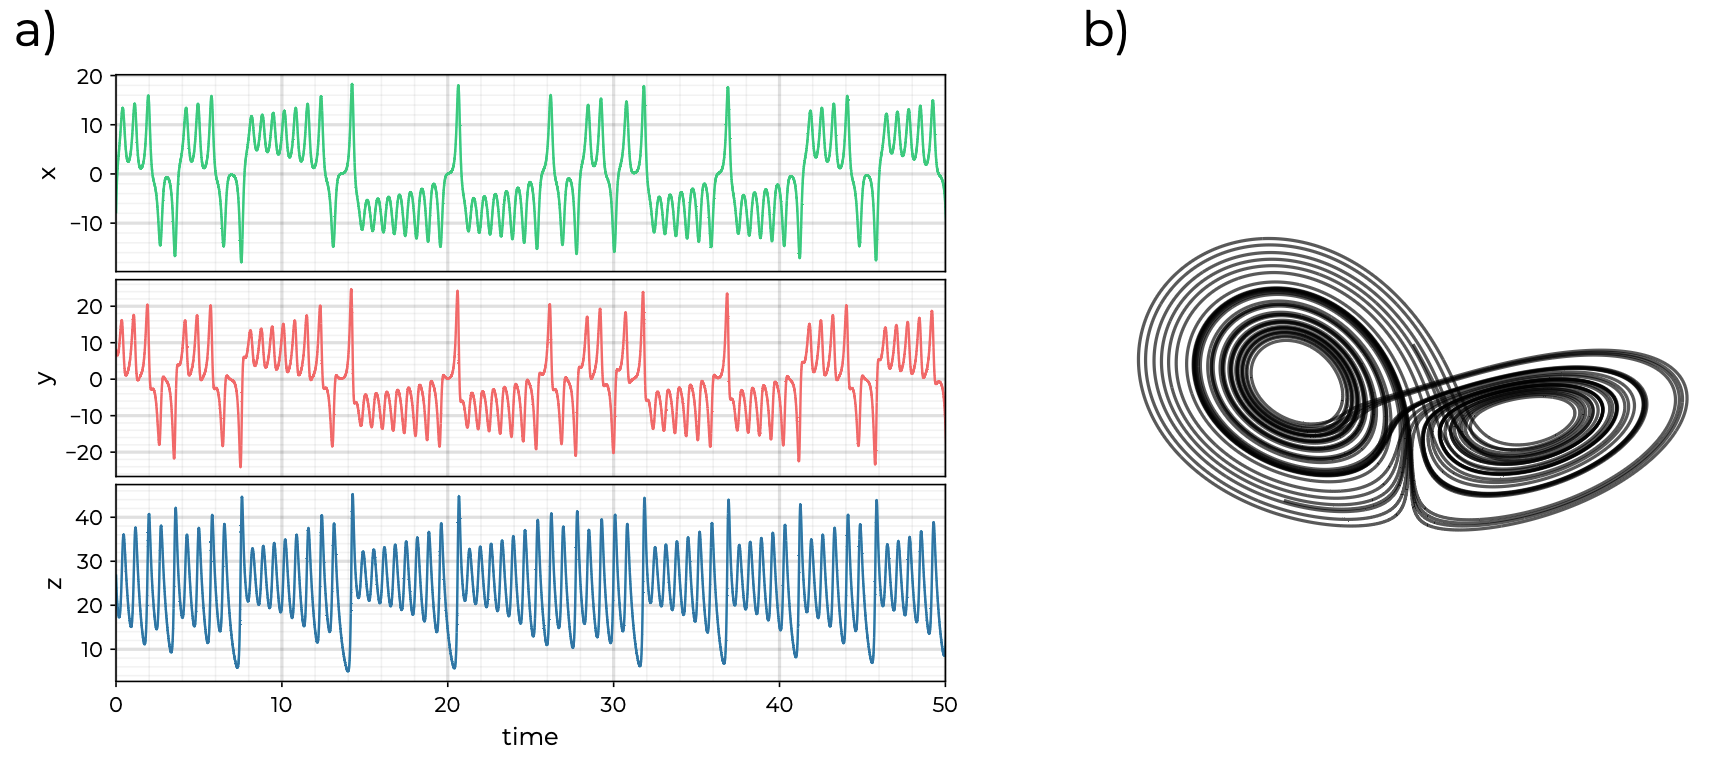
\includegraphics[width=\columnwidth]{havok/0-havok-lorenz/2__lorenz-orig.png}
  \caption{(\textbf{a}) Time series for the $x$, $y$, and $z$ components of the
    Lorenz system. (\textbf{b}) 3-dimensional visualization of the attractor
    formed from $x$, $y$, and $z$ components. We note that there are two clear
    lobes corresponding to the two attractors of the system.}
  \label{fig:lorenz-time-series-orig}
\end{figure}


Given $x(t)$, a $p\times q$ Hankel matrix $\mathbf{H}$ can be formed by concatenating time-shifted
delay embeddings so that:
\begin{equation}
  \mathbf{H} = \begin{bmatrix}
    x_1 & x_2 & \cdots & x_p \\
    x_2 & x_3 & \cdots & x_{p+1} \\
    \vdots & \vdots & \ddots & \vdots \\
    x_q & x_{q+1} & \cdots & x_n
  \end{bmatrix} = \begin{bmatrix}
    x_1 & \mathcal{K}(x_1) \cdots & \mathcal{K}^{p-1}(x_1) \\
    \mathcal{K}(x_1) & \mathcal{K}^2(x_1) \cdots & \mathcal{K}^{p}(x_1) \\
    \vdots & \vdots & \ddots & \vdots \\
    \mathcal{K}^{q-1}(x_1) & \mathcal{K}^q(x_1) \cdots & \mathcal{K}^{n-1}(x_1) \\
  \end{bmatrix}.
\end{equation}
In this form, the relationship of time delay embeddings in $\mathbf{H}$ to the Koopman
operator is clear.

Next we use the SVD to decompose H so that $\mathbf{H} =
\mathbf{U}\mathbf{\Sigma} \mathbf{V}^T$. The columns of $V$ can be interpreted
as \textit{eigen time series} ranked (according to the singular values $\sigma_i
= \mathbf{\Sigma}_{ii}$) by their ability to model the columns of $\mathbf{H}$.
Keeping only the first $r$-many columns of $\mathbf{U}$ and $\mathbf{V}$
therefore provides a low-rank approximation of $\mathbf{H}$ (i.e. more compact)
which will be approximately invariant to the Koopman operator. Instead of
constructing a purely linear model for $\mathbf{V}$, Brunton et al. instead
suggest to fit a linear model for the first $r-1$ components of each
$\mathbf{v}$ and reserve the $r$-th to serve as a source of external forcing.
That is, $\mathbf{A}$ and $\mathbf{B}$ are identified so that
\begin{equation}
  \frac{d}{dt} \mathbf{v}(t) = \mathbf{A}\mathbf{v}(t) + \mathbf{B}f(t)
\end{equation}
where $f(t) = v_r(t)$. Noting that $\dot{\mathbf{v}}$ can be approximated by
$(\mathbf{v}_{i+1}-\mathbf{v}_i)/\Delta t$, then $\mathbf{A}$ and $\mathbf{B}$
are extracted from the first $r-1$ rows and $r$ columns of $\mathbf{\Xi} =
\left(\mathbf{V}_2^T(\mathbf{V_1}^T)^{-1} - \mathbf{I} \right)/ \Delta t$ where
$\mathbf{V}_1$ contains the first n-1 columns of $\mathbf{V}$ while
$\mathbf{V}_2$ includes columns 2 to $n$.

Using an embedding of length $201$ and an $r$ value of $15$ the $\mathbf{A}$ and
$\mathbf{B}$ matrices extracted for the Lorenz system are illustrated in
Figure~\ref{fig:lorenz-A-B-heatmap}. Interestingly, the $\mathbf{A}$
matrix shows a banded diagonal structure.


Time series for the first three components of $\mathbf{v}$ together with their
simulated values under the HAVOK model are are shown in
Figure~\ref{fig:lorenz-havok-embedding}. We note that the embedded attractor
reconstructed from the first three components $v_1$, $v_2$, $v_3$ shown in panel
(b) matches the geometry of the original embedding from Figure~\ref{fig:lorenz-time-series-orig}.

\clearpage
\newpage

\begin{figure}[h]
  \centering
  \includegraphics[width=0.5\columnwidth]{havok/0-havok-lorenz/1b_A-B-sHAVOK.pdf}
  \caption{Fitted operators $\mathbf{A}$ and $\mathbf{B}$ for the Lorenz system
    learned by the HAVOK model corresponding to the linear dynamics and
    intermittent forcing.}
  \label{fig:lorenz-A-B-heatmap}
\end{figure}


\begin{figure}[h]
  \centering
  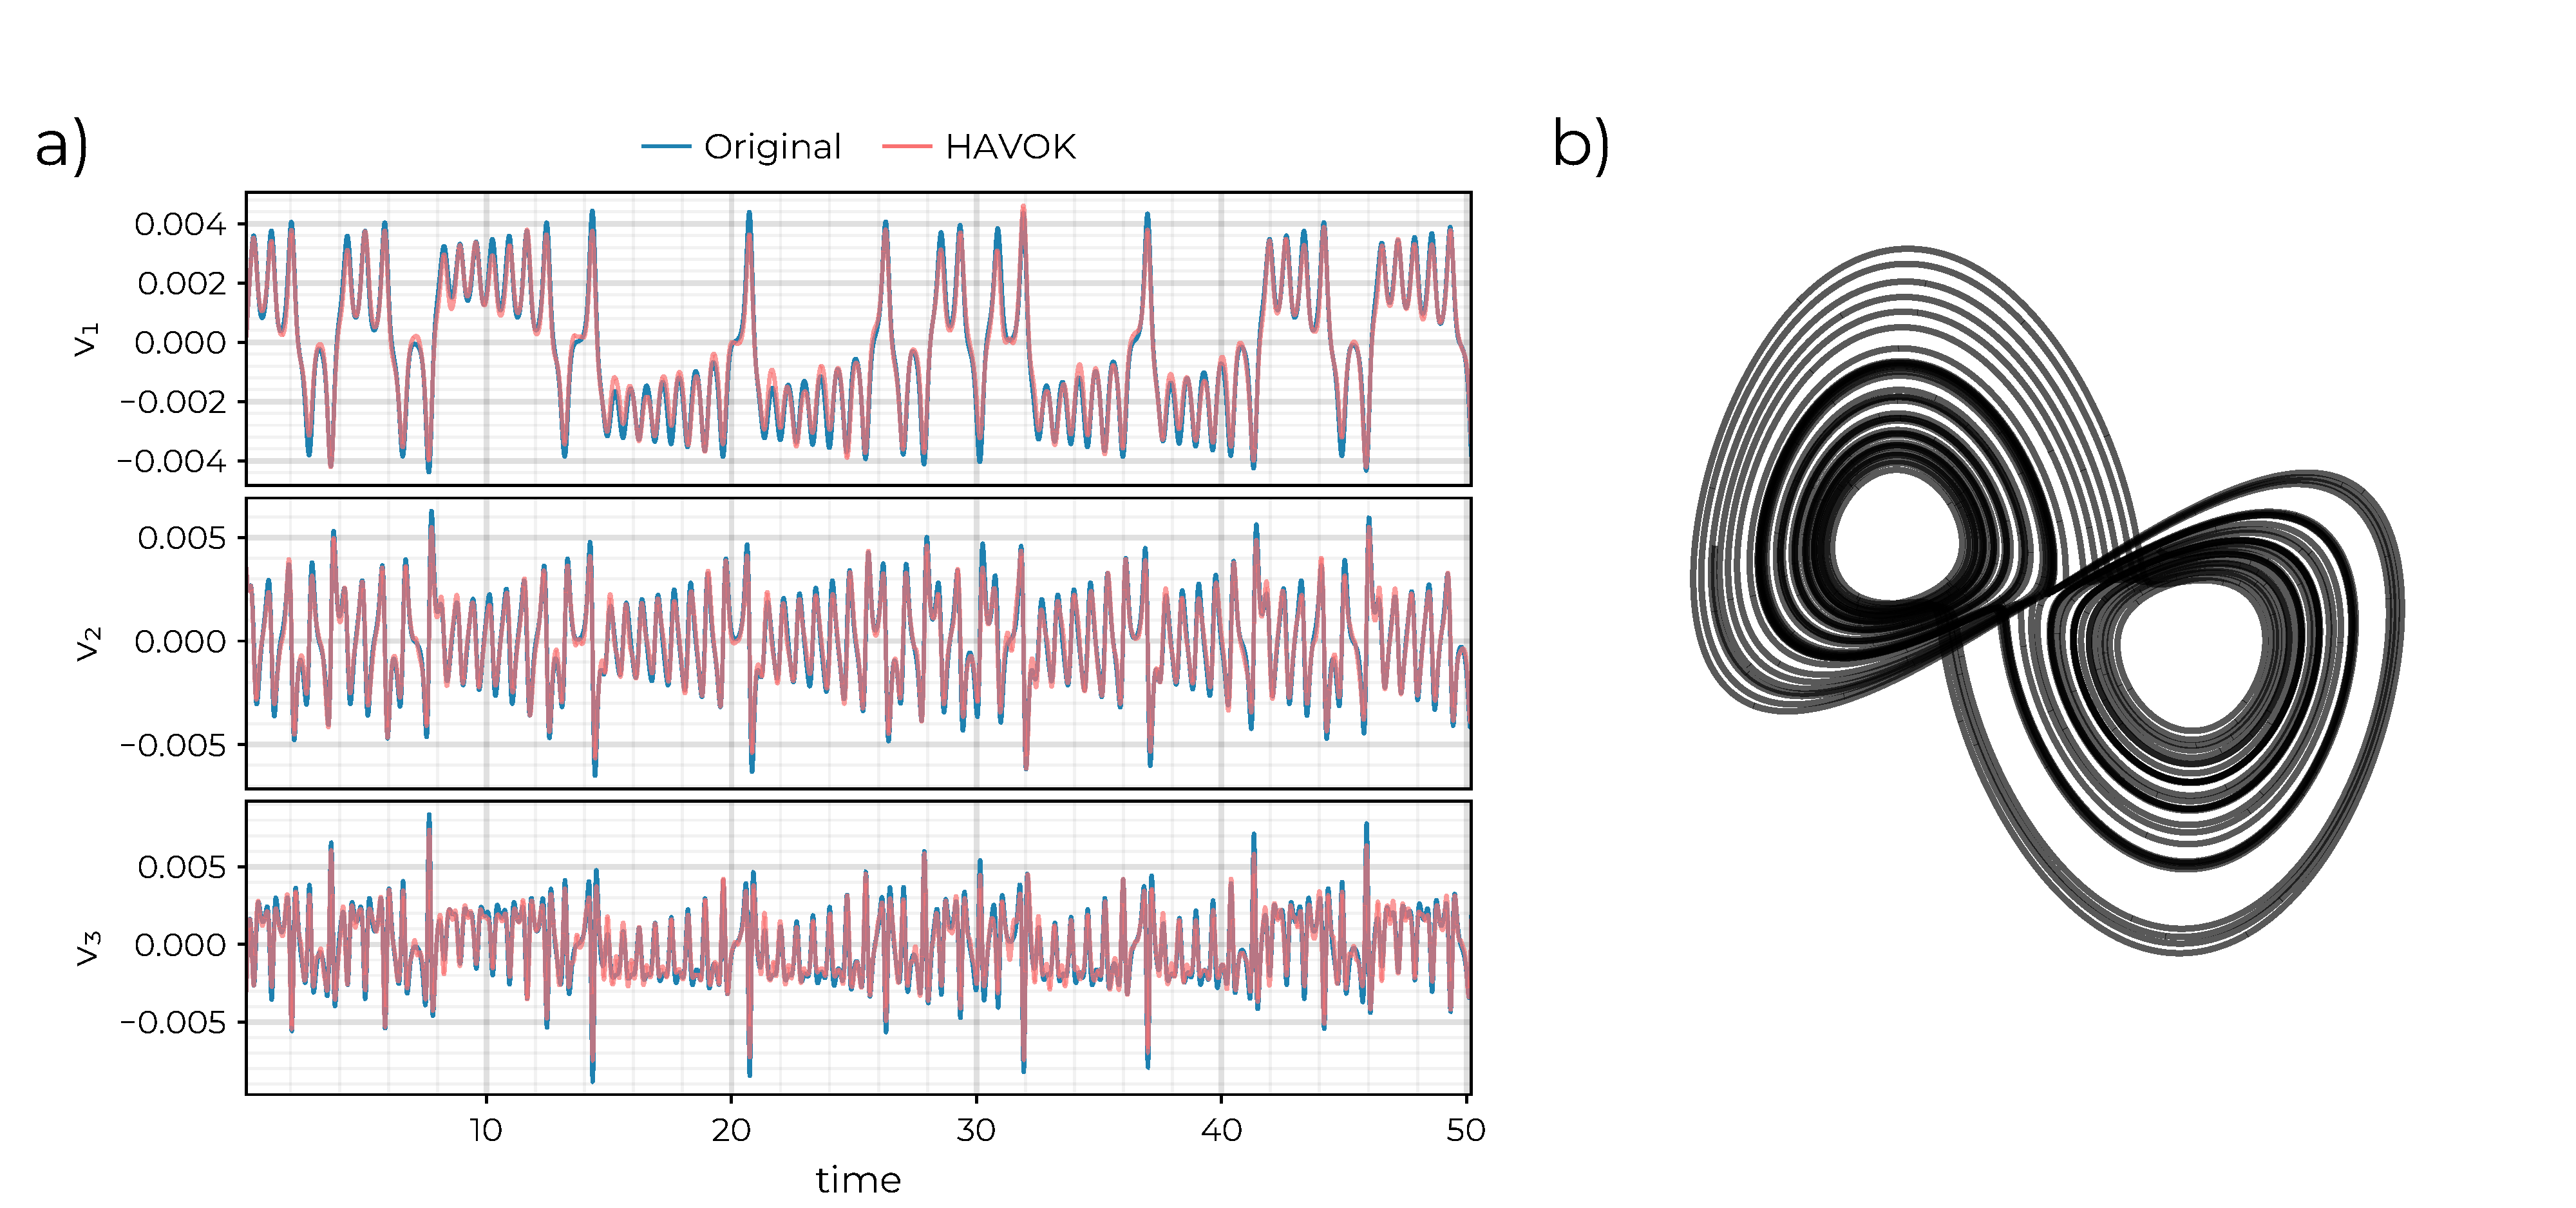
\includegraphics[width=\columnwidth]{havok/0-havok-lorenz/3__havok-embedding.pdf}
  \caption{(\textbf{a}) Time series for first 3 components $v\_i$ of the HAVOK
    model. Original time series for each component are shown in blue. Time
    series predicted by the HAVOK model are overlaid in red. (\textbf(b)) The
    attractor formed by the first 3 embedding coordinates. By Taken's theorem,
    this attractor is diffeomorphic to the original attractor.}
  \label{fig:lorenz-havok-embedding}
\end{figure}


\newpage

Examining the statistics of the extracted forcing term $f(t)=v_r(t)$ reveals
that the effect is indeed consistent with intermittent forcing.
Figure~\ref{fig:lorenz-forcing-stats} illustrates by comparing the estimated
probability density function (PDF) for $v_r(t)$ to a normal distribution
computed using the standard deviation of $v_r$ values. The sharp peak and wide
tails of the PDF reflect the rarity of forcing events.

\begin{figure}[h]
  \centering
  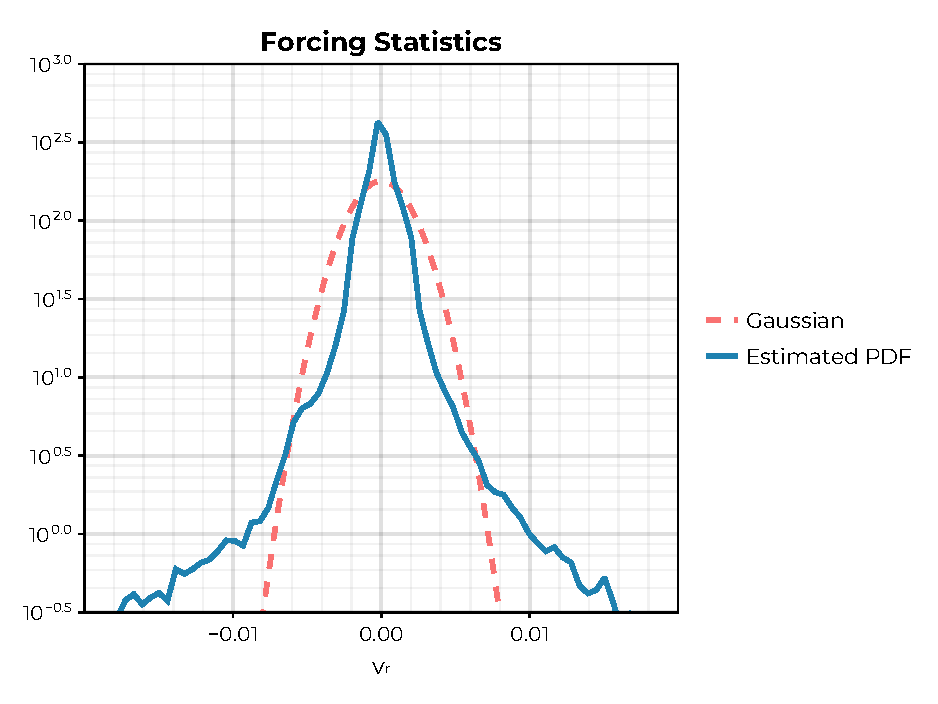
\includegraphics[width=0.75\columnwidth]{havok/0-havok-lorenz/6__forcing-statistics.pdf}
  \caption{Proabability density function for forcing time series learned by the
    HAVOK model. The PDF is compared to a Gaussian fit for the same data. The
    wide tails of the PDF reflect that the forcing is intermittent.}
  \label{fig:lorenz-forcing-stats}
\end{figure}

Identifying forcing values for which $\lvert  v_r \rvert^2$ is above a chosen
threshold clearly identifies lobe-switching in the Lorenz system as illustrated
in Figure~\ref{fig:lorenz-attractor-forcing}.

Using the truncated $\mathbf{U}$ and $\mathbf{\Sigma}$ matrices, the original
time series for $x(t)$ can be reconstructed via the inner product
$\langle \mathbf{\Sigma}\mathbf{u}_{r-1}, \mathbf{v} \rangle$ where $\mathbf{u}_{r-1}$ is the $(r-1)$-th row of $\mathbf{U}$. The reconstructed time
series obtained by integrating the HAVOK model is shown in Figure~\ref{fig:lorenz-reconstruction}.

\clearpage
\newpage

\begin{figure}[h]
  \vspace{-1cm}
  \centering
  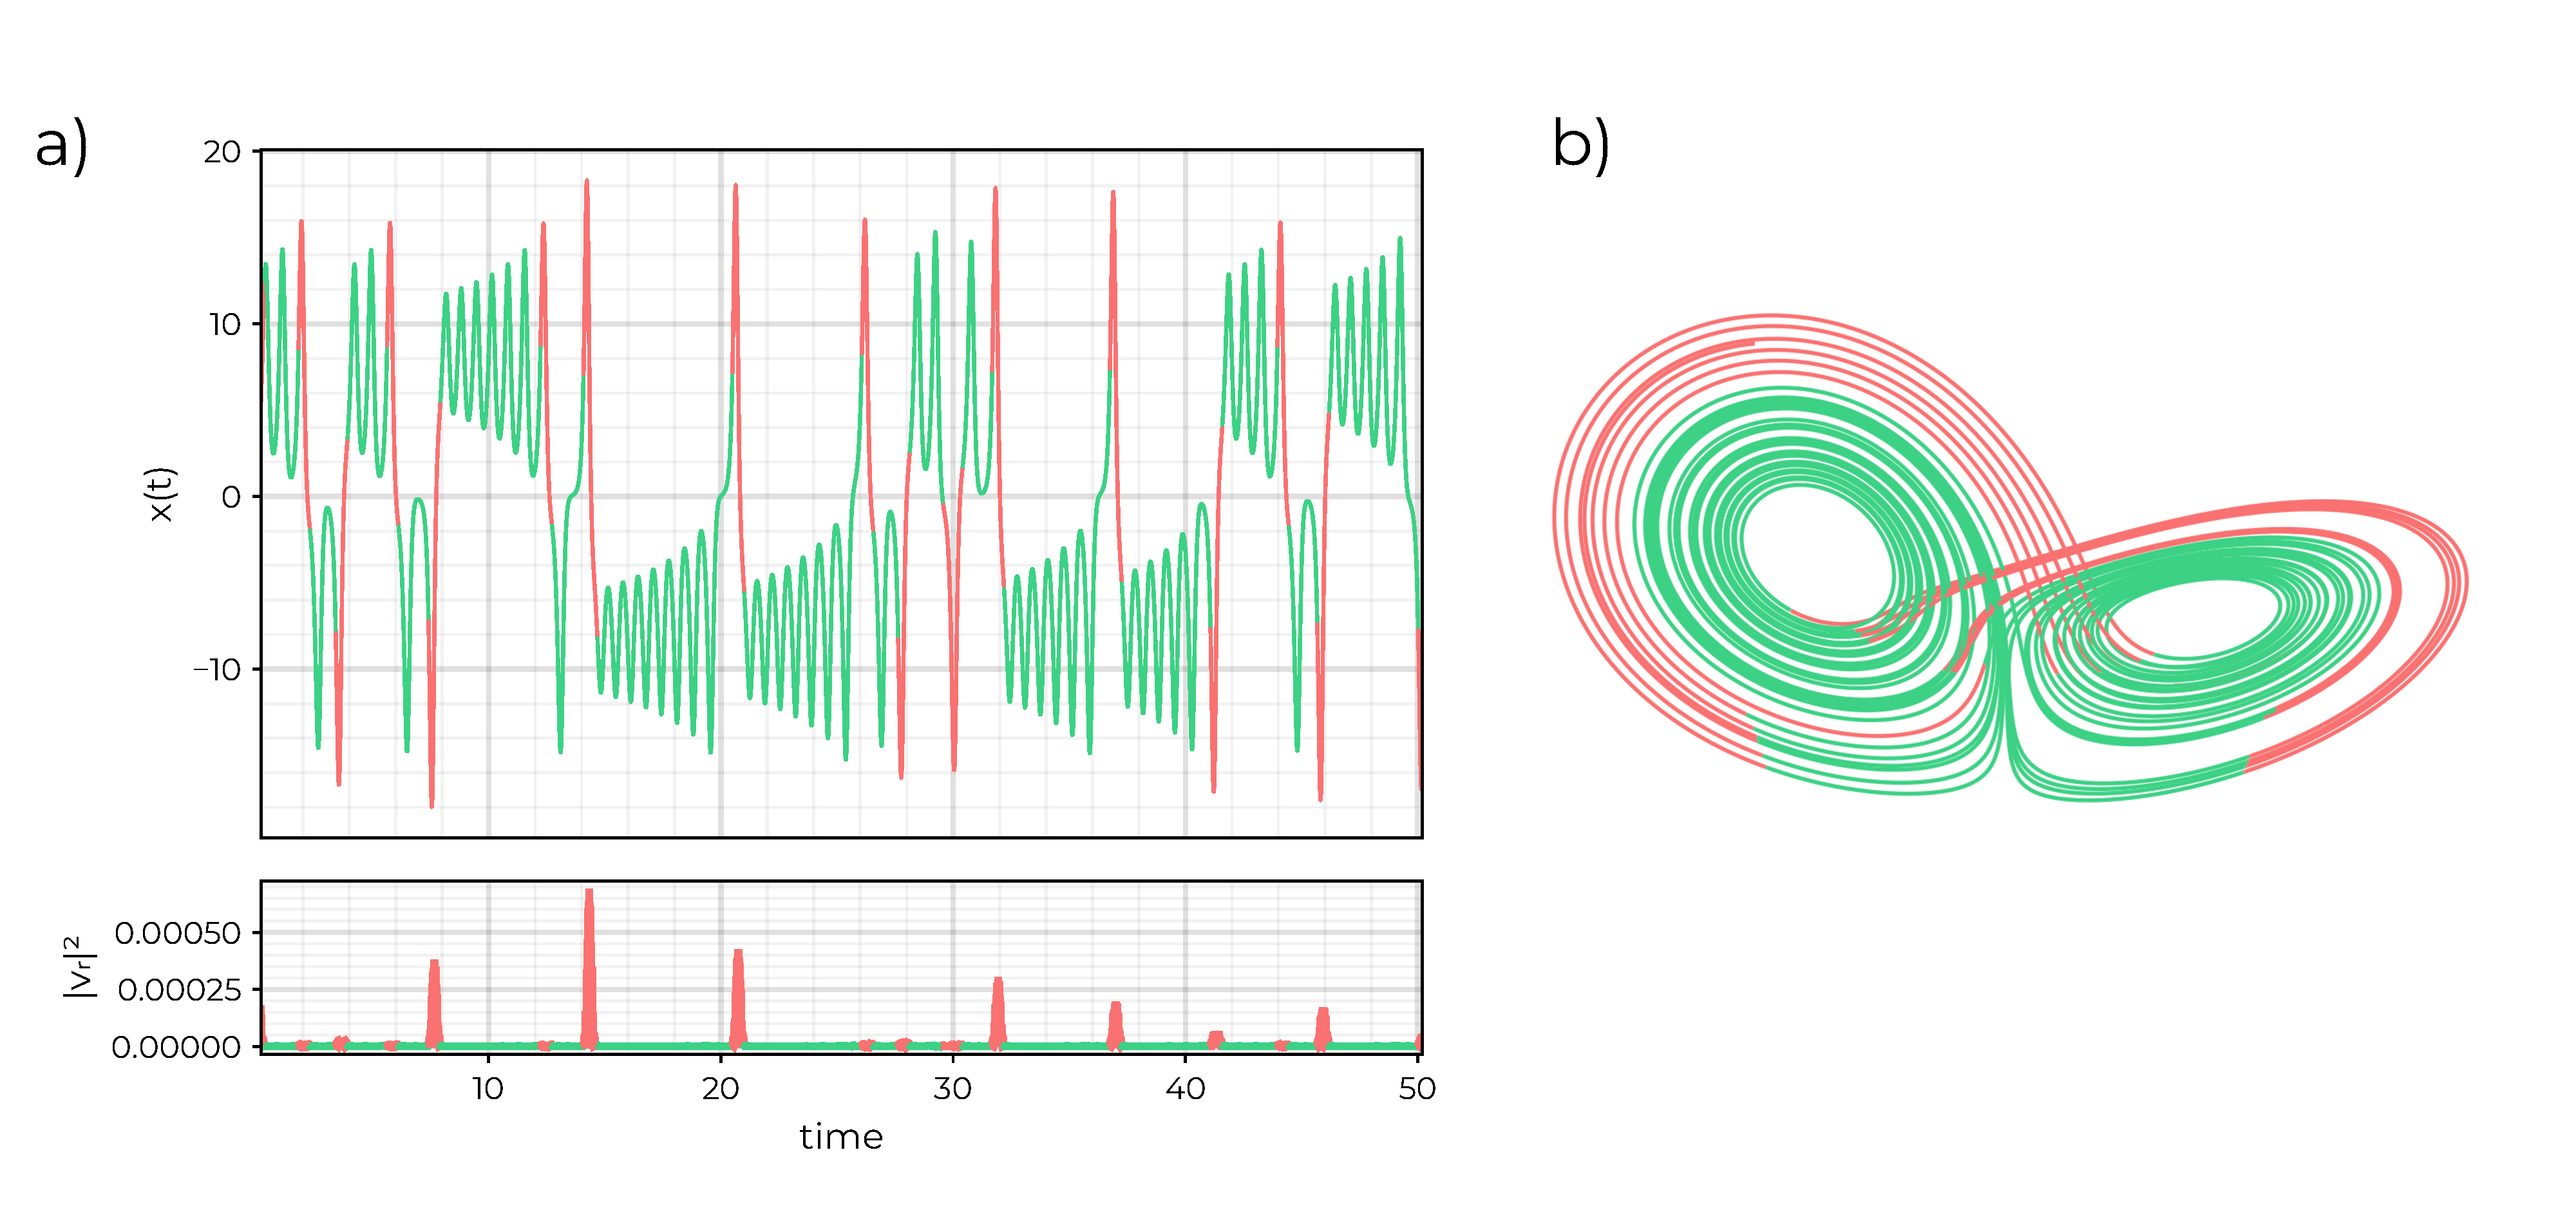
\includegraphics[width=\columnwidth]{havok/0-havok-lorenz/7__attractor-w-forcing.pdf}
  \caption{(\textbf{a}) The original time series $x(t)$ plotted with the squared
  forcing time series $v_r(t)$. Red colors indicate forcing above a chosen
  threshold which accurately identifies lobe-switching events. (\textbf{b}) The
  Lorenz attractor colored using the same scheme.}
  \label{fig:lorenz-attractor-forcing}
  \vspace{-0.5cm}
\end{figure}

\begin{figure}[h]
  \vspace{-0.5cm}
  \centering
  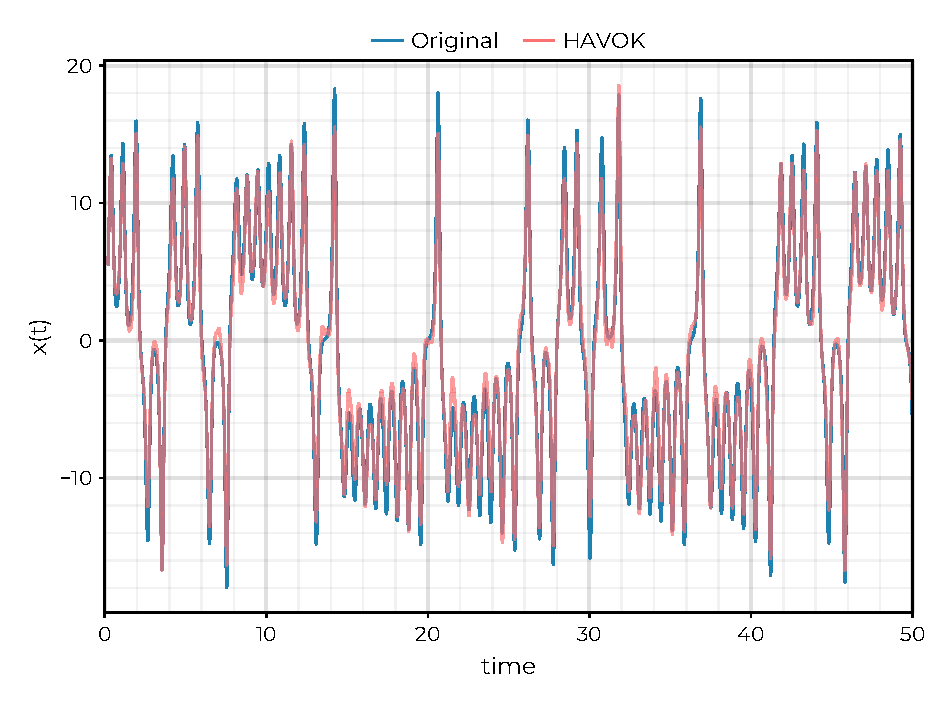
\includegraphics[width=0.8\columnwidth]{havok/0-havok-lorenz/9__timeseries-reconstruction.pdf}
  \caption{The reconstructed time series for $x(t)$ using the fitted HAVOK model.}
  \label{fig:lorenz-reconstruction}
  \vspace{-1cm}
\end{figure}


\newpage

The accuracy of the HAVOK reconstruction for $x(t)$ is encouraging, however we
must note that integrating the HAVOK model forward in time requires that we
provide the values for the external forcing $v_r(t)$. Therefore, forecasts
longer than a single step require that we must separately be able to predict
future values of $v_r(t)$. We note, though, that due to the ranking performed by
the SVD, forcing components extracted from $\mathbf{V}$ tend to be zero centered
with no long term trends (i.e. stationary). Therefore we can expect that
predicting future values of $v_r(t)$ will be a far simpler task than forecasting
the original time series alone.

Additionally, the clear identification of intermittent forcing which proceeds
the lobe switching behavior in the Lorenz systems suggests the extracted forcing
function may provide a useful tool to separate rare pollution episodes from the
typical PM diurnal cycle.

\section{The Frenet-Serret Frame and sHAVOK}

The asymmetric, off-diagonal structure of the $\mathbf{A}$ matrix extracted by
HAVOK for a variety of models lead \cite{havok-diffgeo} to explore the
relationship of the HAVOK model to the local differential geometry of
parameterized curves in $\R^n$. Here we shall briefly consider the description
of such curves using the Frenet-Serret frame which Hirsh et al. used
to motivate a \textit{structured} version of the HAVOK model.

For simplicity, let us consider a smooth curve $\gamma:\R \to \R^3$ describing
a trajectory in three dimensions. At any point along the curve, the
tangent vector $\gamma'(s)$ is identified as
$[\gamma_x'(s), \gamma_y'(s), \gamma_z'(s)]^T$. When
parameterized by arc-length so that the curve moves at unit speed, the tangent
vector is denoted by $\hat{t}(s)=\gamma'(s)$. Similarly, the \textit{curvature},
$\kappa(s)$ of $\gamma$ is defined by  $\alpha''(s) = \kappa(s)\hat{n}(s)$ where
$\hat{n}$ is the unit normal vector to $\gamma$ at $s$. Finally, taking the
cross product between the two yields the unit binormal vector $\hat{b}(s) =
\hat{n}(s) \times \hat{t}(s)$.

Since $\hat{b}\cdot\hat{b}=1$, it follows by differentiation that $\hat{b}'
\perp \hat{b}$. Additionally, the product rule yields, $\hat{b}' = \hat{n}' \times
\hat{t}$ so that $\hat{b}' \perp \hat{t}$. Since $\hat{b}'$ is perpendicular to
both $\hat{b}$ and $\hat{t}$, it follows that
\begin{equation}
  \hat{b}'(s) = - \tau(s)\hat{n}(s)
\end{equation}
where we have defined the torsion $\tau(s)$. The vectors $\left\{\hat{t},
    \hat{n}, \hat{b} \right \}$ form an orthonormal basis at each point of the
curve $\gamma$. Finally, we note that $\hat{n}  = \hat{t} \times \hat{b}$ so
that
\begin{align}
  \hat{n}'(s) &= \hat{t}'(s)\times \hat{b}(s) + \hat{t}(s) \times \hat{b}'(s) \\
              &= \kappa(s)\hat{n}(s)\times\hat{b}(s) + \hat{t}(s) \times (-\tau(s)\hat{n}(s)) \\
  &= - \kappa(s)\hat{t}(s) + \tau(s)\hat{b}(s)
\end{align}
which in matrix form becomes
\begin{equation}
  \begin{bmatrix} \hat{t}' \\ \hat{n}' \\ \hat{b}' \end{bmatrix} = \begin{bmatrix}
    0 & \kappa(s) & 0 \\
    - \kappa(s) & 0 & \tau(s) \\
    0 & -\tau(s) & 0
    \end{bmatrix} \begin{bmatrix} \hat{t} \\ \hat{n} \\ \hat{b} \end{bmatrix}
\end{equation}

For $n$ dimensional curves, the approach can be extended by using the
Gram-Schmidt procedure to produce an orthonormal basis from the $n$-derivatives
of $\gamma(s)$. The generalization leads to an expression of the form
\begin{equation}
    \begin{bmatrix} \hat{e}_1' \\ \hat{e}_2' \\ \vdots \\ \hat{e}_n' \end{bmatrix} = \begin{bmatrix}
    0 & \kappa_1(s) &  & 0 \\
    -\kappa_1(s) & \ddots & \ddots & \\
     & \ddots & 0 & \kappa_{n-1}(s) \\
     0 &  & -\kappa_{n-1}(s) & 0 \\
    \end{bmatrix} \begin{bmatrix} \hat{e}_1 \\ \hat{e}_2 \\ \vdots \\ \hat{e}_n \end{bmatrix}
\end{equation}
where $\hat{e}_i$ are the unit vectors resulting from the Gram-Schmidt process
and $\kappa_i(s)$ are called \textit{generalized curvatures}.

This structure clearly resembles the form of $\mathbf{A}$ identified in
Figure~\ref{fig:lorenz-A-B-heatmap}. Based on this, Hirsh et al. realized that
maintaining the orthogonality of the components $\mathbf{v}(t)$ when fitting the
HAVOK model reinforces this local structure. This led them to develop a
\textit{structured}-HAVOK (sHAVOK) method which fits $\mathbf{A}$ and
$\mathbf{B}$ by first computing two separate Hankel matrices $\mathbf{H}_1$ and
$\mathbf{H}_2$ containing the first $n-1$ columns of $\mathbf{H}$ and
columns 2 through $n$, respectively. Then, the SVD is taken for each separate
Hankel matrix yielding $\mathbf{V}_1$ and $\mathbf{V}_2$ which result from time
shifted data, but unlike the original formulation, are guaranteed to maintain
the orthogonality of both $\mathbf{V}_1$ and $\mathbf{V}_2$. Finally,
$\mathbf{A}$ and $\mathbf{B}$ are obtained by computing $\mathbf{\Xi} =
(\mathbf{V}_2^T\mathbf{V}_1 - \mathbf{I})/\Delta t$ and selecting $\mathbf{A}$
and $\mathbf{B}$ from the first $r-1$ rows and $r$ columns. We employ this
updated approach for the analysis of PM 2.5 time series data in the rest of this
chapter.

\section{Study Overview and Extensions to HAVOK}

To examine the ability of structured HAVOK for PM modeling and
forecasting, we identified a set of PM 2.5 measurements collected the IPS7100 sensor
at a site in Plano, Texas during August of 2023. This time period was specifically
chosen as it was in the middle of a dry stretch of zero precipitation in the
North Texas region. Because humidity can induce hygroscopic growth of
particulates leading to overestimation of particle concentrations, most federal
equivalent methods utilize heating elements to pre-process PM samples
before evaluating their abundance. However, the inclusion of heating elements
dramatically increases sensor complexity leading to increased cost, increased
power requirements, and lower sampling rates. Therefore to fairly assess the
HAVOK model, we shall consider here 10 days of continuous, precipitation-free
measurements for PM 2.5 averaged to a 10-second time resolution to reduce
sampling noise. The full time series is visualized in
Figure~\ref{fig:pm-timeseries-orig}. We note that this particular example shows
the typical diurnal cycle with peaks  generally falling in the afternoon
to early evening hours. Additionally, this sample dataset includes a number of
sharp spikes which will allow us to asses the utility of the forcing function
learned by the HAVOK model.

\begin{figure}[h]
  \centering
  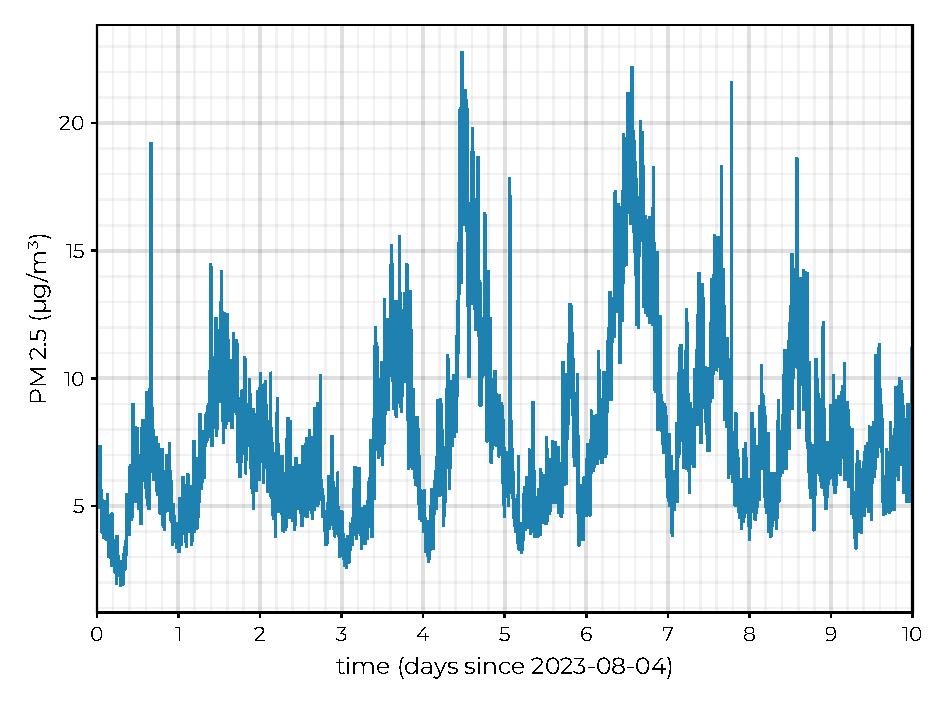
\includegraphics[width=0.8\columnwidth]{havok/1-havok-pm/1__timeseries-full-short.pdf}
  \caption{Time series of PM $2.5$ measurements from Central Hub 4 located in
    Planeo, Tx starting on 2023-08-04. This time series was selected during the
    long period of no precipitation during 2023 in order to limit the impact of
    hygroscopic growth on observed values. Note the occasional, thin vertical
    spikes corresponding to acute pollution events.}
  \label{fig:pm-timeseries-orig}
\end{figure}

Previous application of the HAVOK model utilized a single forcing function
identified via the $r$-th column of $\mathbf{V}$. This is reinforced by the
structure suggested from the Frenet-Serret for which all matrix entries beyond
the $r$-th column \textit{should} be zero. However, the fitting procedure of the
HAVOK and sHAVOK models does not enforce this requirement. Indeed for the
examples presented in \cite{brunton-havok-orig} and \cite{havok-diffgeo}, the
vectors $\mathbf{B}$ had more than one non-zero entry. Therefore, we extend the
model so such that
\begin{equation}
  \dot{\mathbf{v}}(t) = \mathbf{A}\mathbf{v}(t) + \mathbf{B}\mathbf{f}(t)
\end{equation}
where $\mathbf{f}$ is now a vector of forcing terms corresponding to $n$ columns
of $\mathbf{V}$ past column $r$. This promotes $\mathbf{B}$ to a matrix but
leads to no further modifications to the fitting procedure.

To extend the HAVOK model to enable forecasting, we make one additional
modification involving how the model is integrated. In the codes developed for
\cite{brunton-havok-orig, havok-diffgeo}, the authors used a standard
integration method for control systems which assumes that the forcing
function $f(t)$ is piecewise linear between each time-step. This is a reasonable
assumption as the values of the forcing function are obtained at the same
temporal resolution as the original time series sampling rate. To utilize more
complicated integration schemes, one must interpolate the forcing function
values to enable their evaluation at points between sample times. However, in
both papers the authors note that the forcing function values precede large
changes in the original time series. We therefore adopt a simpler integration
approach which assumes only that forcing function values are
\textit{piecewise-constant} between sample points. This means that the HAVOK
model can be integrated from $t$ to $t+\Delta t$ by solving
\begin{equation}
  \begin{cases}
    \dot{\mathbf{v}} = \mathbf{A}\mathbf{v}(t) + \mathbf{B}\mathbf{f}(t) \\
    \dot{\mathbf{f}}(t) = 0
  \end{cases}
\end{equation}
Since $\mathbf{A}$ and $\mathbf{B}$ are constant matrices, the solution can be
written exactly using matrix exponentials so that
\begin{equation}
  \begin{bmatrix} \mathbf{v}(t+\Delta t) \\ \mathbf{f}(t+\Delta t) \end{bmatrix} = \exp \left(  \begin{bmatrix}
    \mathbf{A}\Delta t & \mathbf{B} \Delta t \\
    0 & 0
  \end{bmatrix} \right) \begin{bmatrix} \mathbf{v}(t) \\ \mathbf{f}(t) \end{bmatrix}
\end{equation}

The overall accuracy of the HAVOK model is strongly determined by the chosen
cutoff value used to truncate $\mathbf{V}$ after taking the SVD of
$\mathbf{H}_1$ and $\mathbf{H}_2$. Furthermore, because forcing terms correspond
to singular vectors which explain little of the total variance in $\mathbf{H}_1$
and $\mathbf{H}_2$, it is reasonable to expect that this approximation will be
valid. Indeed for the Lorenz system example shown
Figure~\ref{fig:lorenz-reconstruction}, we used this integration scheme to
evaluate the HAVOK model.

A natural consequence of this choice is that single-step predictions of the
HAVOK model no longer require future knowledge of the forcing function. That is,
$\mathbf{v}(t+\Delta t)$ only depends on the current state $\mathbf{v}(t)$ and
the current forcing values $\mathbf{f}(t)$. Furthermore, multi-step
predictions for the forcing terms can now leverage both the current delay-embedding of
time series values \textit{and} the value at the next time step. We use this to
motivate a simple regression model for forecasting $\mathbf{f}$ thereby enabling
forecasting for PM 2.5 beyond single-step forecasts.

A principle component decomposition of a Hankel matrix for the PM 2.5 data 
using an embedding of length 100 is shown in Figure~\ref{fig:pm-timeseries-pca}.
Included in the plot is a horizontal line indicating an explained variance of
$1\%$.

\begin{figure}[h]
  \centering
  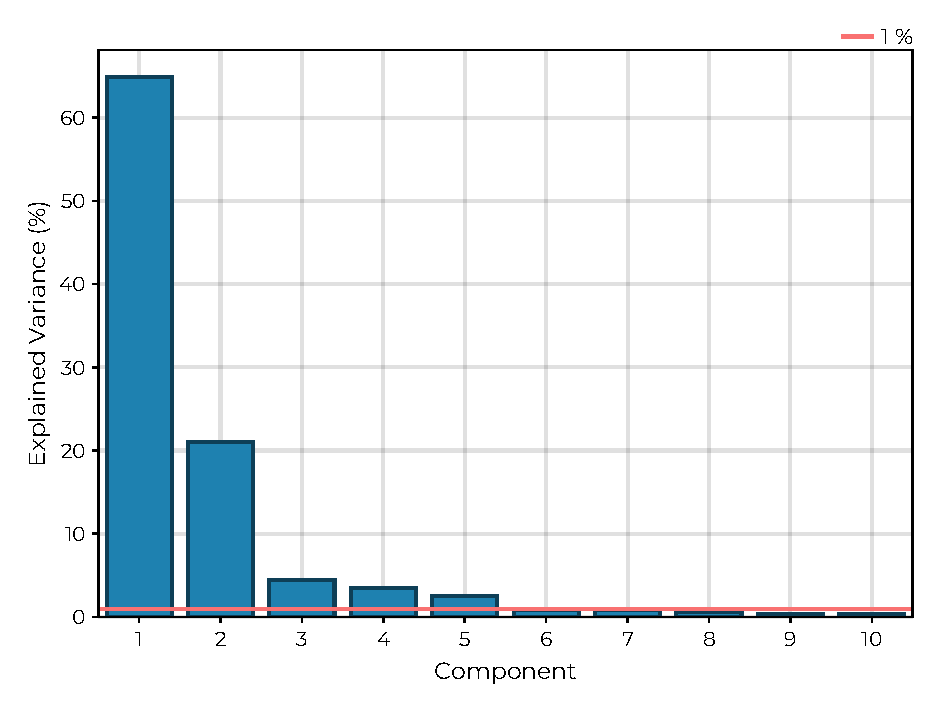
\includegraphics[width=0.7\columnwidth]{havok/1-havok-pm/1__pca-explained-variance.pdf}
  \caption{Explained variance of components from a principal component
    decomposition of the PM 2.5 time series sorted in decreasing order. A red
    line is superimposed indicating a $1\%$ explained variance. All components
    past the sixth contribute less than $1\%$ to the total explained variance. }
  \label{fig:pm-timeseries-pca}
\end{figure}

While the choice of an embedding length of $100$ is arbitrary, these values
suggest that a state vector of at length $3$ should be explored for our HAVOK
models. Based on these indications, we performed a comprehensive parameter sweep,
training multiple HAVOK models for embedding lengths ranging from $N=30$ to
$N=360$, for state vectors of length $r=3$ to $r=25$ and for forcing functions
of length $n=1$ to $n=5$ subject to the constraints that $r>n$ and $r+n \leq N$
for each model.

To evaluate the model performance, the data was split into two distinct time
series corresponding to the first 7 days and the final 3 days of the time
series, respectively. This train-test split is visualized in
Figure~\ref{fig:pm-train-test-split}. We note that unlike the random splits used
for the supervised regression in Chapter~\ref{ch:robot-team-supervised}, it is
critical to separate the data into  disjoint time series to prevent data leakage
from future values into the training set during model fitting.

To evaluate each model, the RMSE and MAE are computed between the original PM
2.5 data and the reconstructed values obtained by integrating the HAVOK model
starting at the first value of the test set. Using these results, we then train
a final HAVOK model with the identified hyperparameter values and explore the
resulting time series.

\begin{figure}[h]
  \centering
  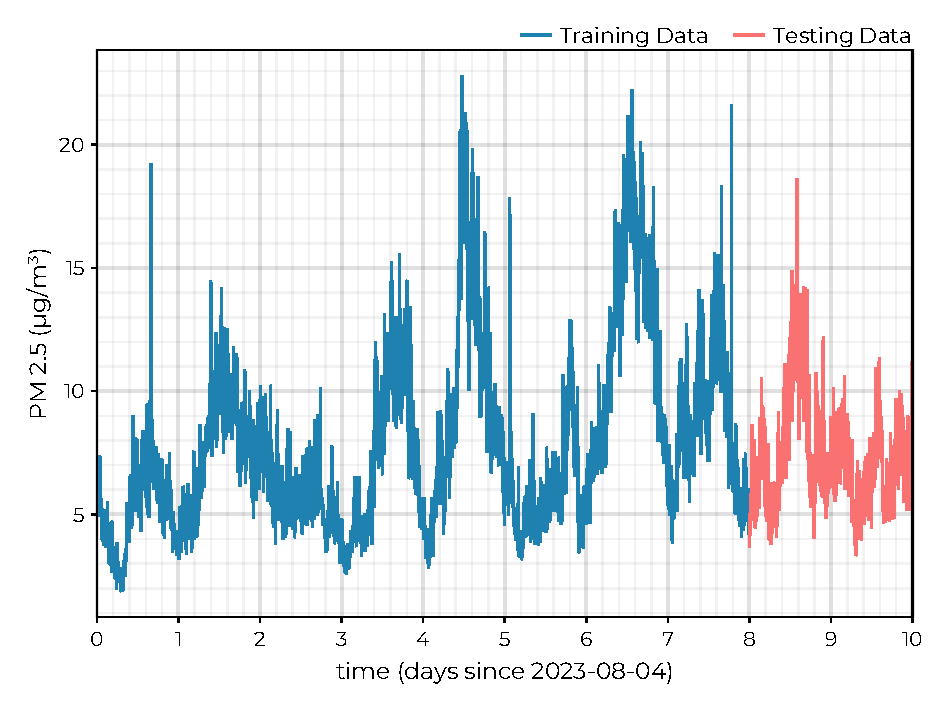
\includegraphics[width=0.8\columnwidth]{havok/1-havok-pm/1b__train-test-timeseries-short.pdf}
  \caption{Train-test split used for training the HAVOK model. To prevent data
    leaks, i.e. information from the future being incorporated into forecasts,
    the data was partitioned into two continuous sets to be used separately for
    model fitting and evaluation.}
  \label{fig:pm-train-test-split}
\end{figure}

\section{Results}

A comparison of the trained HAVOK models for the hyperparameter sweep over
embedding length, sate vector length, and number of forcing terms is presented
in Table~\ref{tab:havok-fit-results}. The table includes the top 10 performing
models ranked by their RMSE on the testing set as well as the top three models
with only a single forcing function which fell further down the list. The best
model utilized a delay embedding of length $30$ corresponding to a 5 hour
window, with a state vector of length $6$ and $5$ total forcing functions. Based
on these results, incorporating additional forcing terms clearly leads to an
improved model.

\begin{table}[h]
  \caption{Results of HAVOK model hyperparameter search. Models were trained
    varying the embedding size ($N$), number of state variables $(r)$, and
    number of forcing terms ($n$). The top 10 models are presented here as
    evaluated by their RMSE and MAE values ranked in descending order.
    Additionally the top 3 models with $n=1$ are included for comparison.}
  \label{tab:havok-fit-results}
  \centering
  \begin{tabular}{ccccc} \hline
    \textbf{N} & \textbf{r} & \textbf{n} & \textbf{RMSE}  & \textbf{MAE} \\ \hline
    $30$ & $6$ & $5$ & $0.216703$ & $0.155912$ \\
    $45$ & $10$ & $5$ & $0.3649$ & $0.268842$ \\
    $30$ & $6$ & $4$ & $0.472797$ & $0.397746$ \\
    $45$ & $8$ & $5$ & $0.487448$ & $0.358938$ \\
    $30$ & $7$ & $5$ & $0.583654$ & $0.518485$ \\
    $30$ & $8$ & $5$ & $0.58551$ & $0.428986$ \\
    $30$ & $7$ & $4$ & $0.586575$ & $0.520145$ \\
    $30$ & $8$ & $4$ & $0.610296$ & $0.447673$ \\
    $30$ & $8$ & $3$ & $0.620928$ & $0.455369$ \\
    $60$ & $12$ & $5$ & $0.697797$ & $0.507499$ \\
    $\vdots$ & $\vdots$ & $\vdots$ & $\vdots$ & $\vdots$ \\
    $105$ & $3$ & $1$ & $1.48989$ & $1.09792$  \\
    $120$ & $3$ & $1$ &  $1.58473$ & $1.1494$ \\
    $180$ & $5$ & $1$ & $1.77659$ & $1.29506$
  \end{tabular}
\end{table}


Using these parameters, a final HAVOK model was trained. The structure of the
$\mathbf{A}$ and $\mathbf{B}$ matrices corresponding to the linear and forcing
components of the model are visualized in the first panel of
Figure~\ref{fig:pm-havok-operators}. The $\mathbf{A}$ matrix includes the
expected diagonal structure while the forcing terms in $\mathbf{B}$ decrease
with each column. The eigenvalues of $\mathbf{A}$ are also included in
Figure~\ref{fig:pm-havok-operators} where it can be clearly seen that no
eigenvalue has any postive, real component. This reflects that the HAVOK model
is stable, at least during periods with little forcing.

\begin{figure}[h]
  \vspace{-2cm}
  \centering
  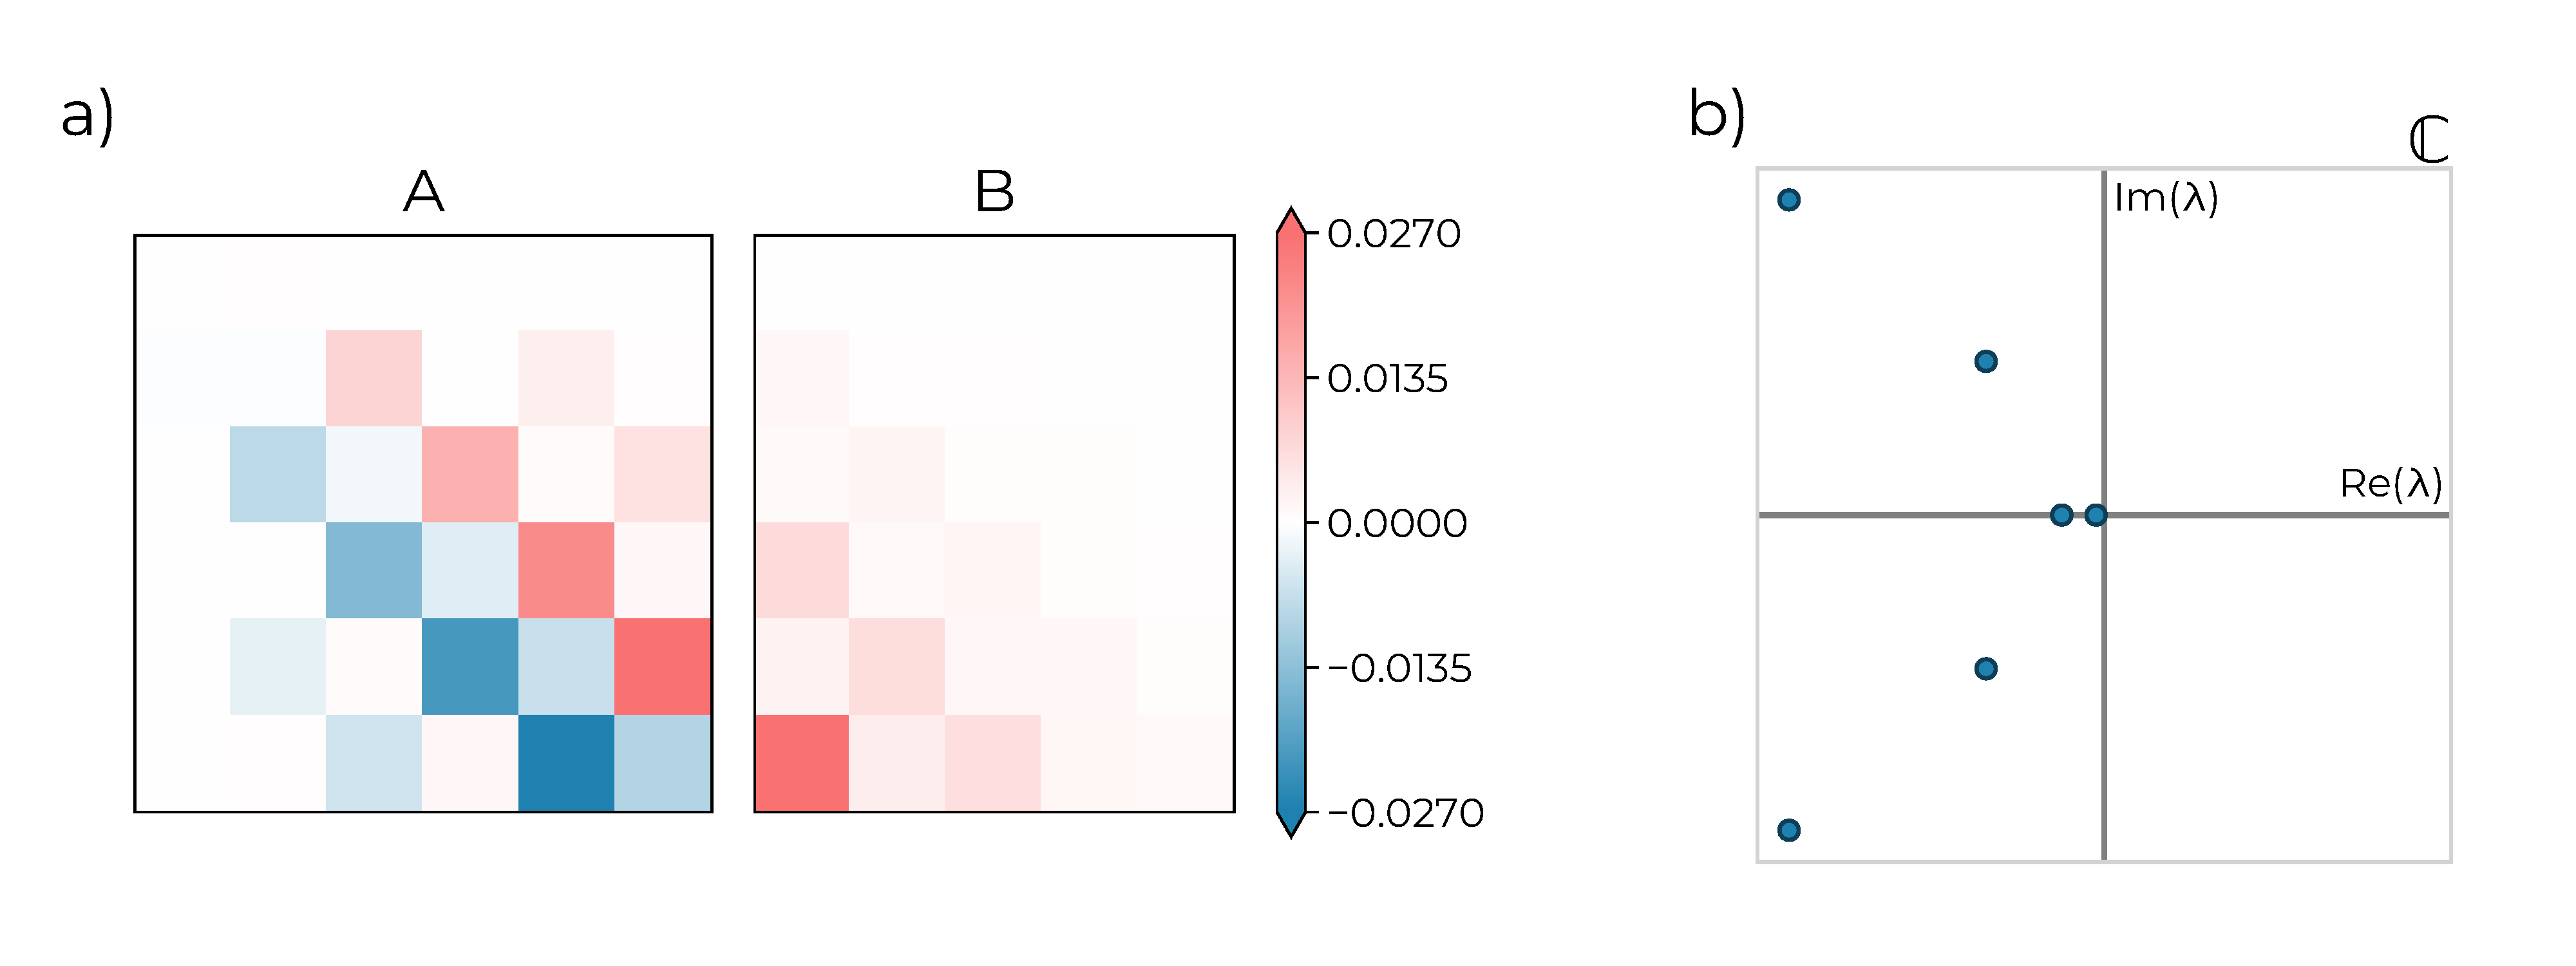
\includegraphics[width=0.9\columnwidth]{havok/2-havok-eval/2__model-terms.pdf}
  \caption{(\textbf{a}) Operators learned by the HAVOK model with $r=6$ and
    $n=5$. We note that the $\mathbf{A}$ matrix displays the expected banded
    diagonal  structure. Additionally, the values of the forcing matrix
    $\mathbf{B}$ decrease with each column. (\textbf{b}) Eigenvalues of the
    learned HAVOK operator $\mathbf{A}$ visualized in the complex plane. We note
    that no eigenvalues had any postive real component reflecting the model's
    stability for integration over long time periods.}
  \label{fig:pm-havok-operators}
\end{figure}

The reconstructed time series generated by integrating the training HAVOK model
for both the training and testing sets is shown in
Figure~\ref{fig:pm-havok-predictions}. Here the external forcing terms,
$\mathbf{f}(t)$ are provided during the integration in order to demonstrate the
stability of the HAVOK model. We note that the final RMSE of $0.217$ $\mu g/m^3$
is at the level of sensor uncertainty for 10-second data.

The inset figure within Figure~\ref{fig:pm-havok-predictions} shows a subset of
the time series for a 4-hour window further showcasing the excellent agreement
between the original data and the trained model. The model is also able to
accurately capture the intermittent PM spikes which occur throughout the
duration of the time series.

\begin{figure}[h]
  \centering
  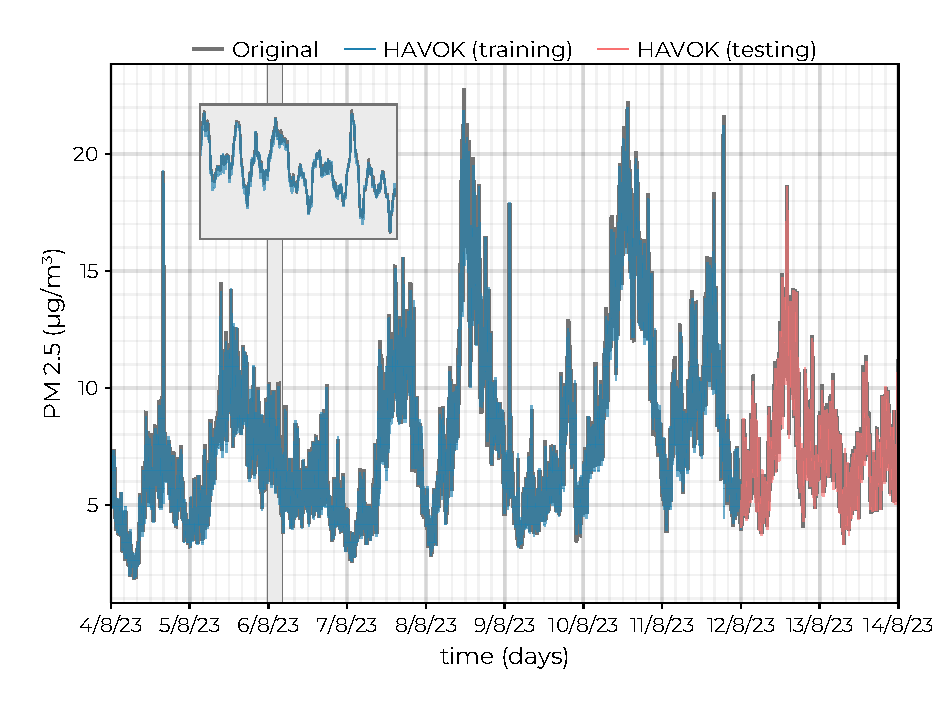
\includegraphics[width=0.75\columnwidth]{havok/2-havok-eval/1__predicted-ts-training.pdf}
  \caption{Time series predicted by HAVOK model with forcing functions provided.
  Inset into the figure is a subset of the }
  \label{fig:pm-havok-predictions}
\end{figure}


\subsection{Forcing Statistics and Outlier Detection}

As previously mentioned, one goal for the HAVOK model is to utilize the
extracted forcing functions to identify intermittent pollution spikes.
Figure~\ref{fig:pm-forcing-stats} plots the estimated probability density
function for the first forcing term, $f_1(t)$ compared to a Gaussian fit using
the standard deviation of $f_1(t)$ across the time series. On the log-scale, the
wide tails of the distribution confirm that the extracted forcing activates
intermittently as intended.

\begin{figure}[h]
  \centering
  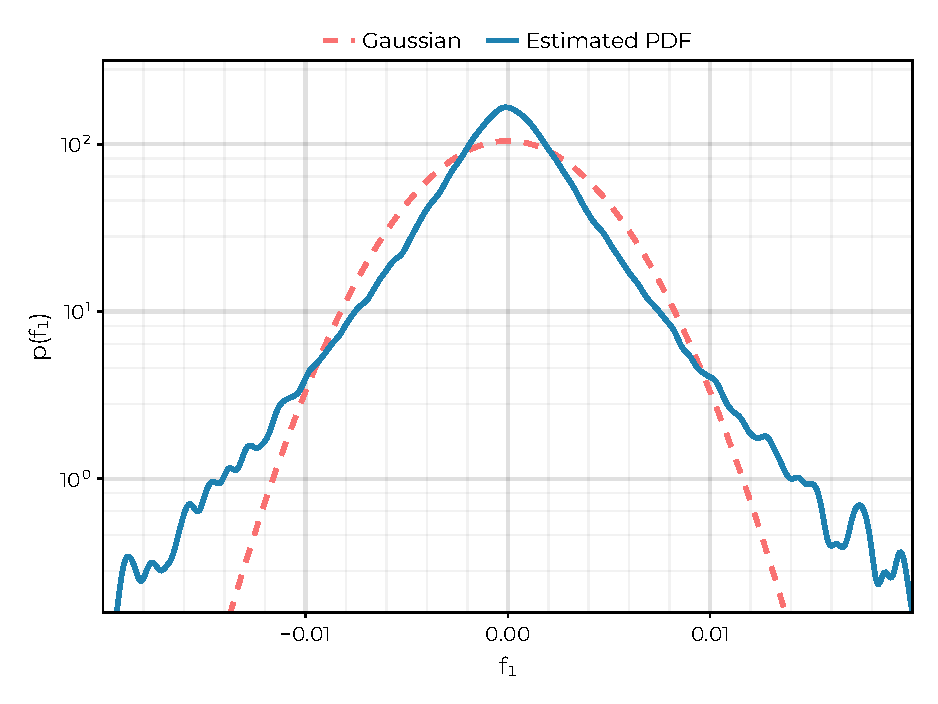
\includegraphics[width=0.65\columnwidth]{havok/2-havok-eval/4__forcing-statistics.pdf}
  \caption{Probability density function evaluated for the first forcing function
  compared to a zero-mean Gaussian distribution fit to the forcing data. The
  wide tails of the estimated distribution reflect the intermittent activation
  of forcing.}
  \label{fig:pm-forcing-stats}
\end{figure}

Following the Lorenz system example from \cite{brunton-havok-orig}, we utilize
thresholded values of $f_1(t)$ to identify intermittent spikes in the original
PM 2.5 time series. The result is visualized in
Figure~\ref{fig:pm-time-series-w-forcing} which includes both the original PM
2.5 data together with the time series for $\lvert  f_1(t) \rvert^2$. A cutoff
threshold of $0.0006$ accurately extracts three pollution spikes which were
observed on the 4th, 9th, and 11th of August, respectively. Lower threshold
values an be used to further identify smaller spikes which occur throughout each day.

\begin{figure}[h]
  \centering
  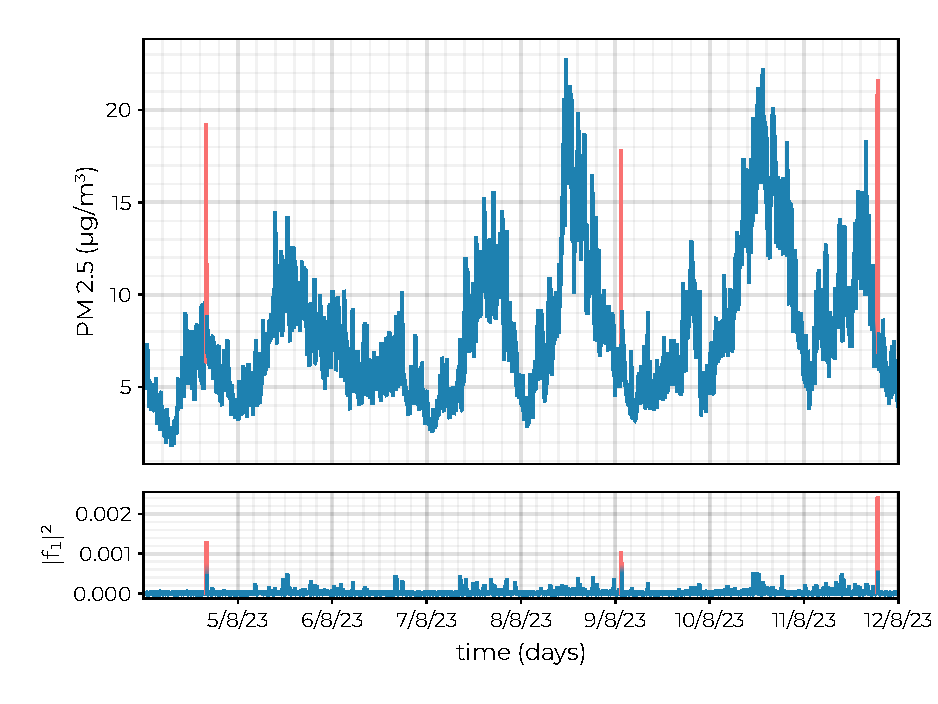
\includegraphics[width=\columnwidth]{havok/2-havok-eval/6__timeseries-with-forcing.pdf}
  \caption{The original PM 2.5 time series plotted together with the squared
    value of the first forcing function, $\lVert  f_1(t) \rVert^2$. By
    thresholding the values of $f_1$, the intermittent PM spikes are easily
    identified. }
  \label{fig:pm-time-series-w-forcing}
\end{figure}


\subsection{Forecasting with HAVOK}

Forecasting with the HAVOK model shifts the problem to modeling
future values of the forcing function. At face value, this may not provide any
obvious benefit, however the time series corresponding to forcing functions
tend to be stationary since the SVD organizes singular vectors by decreasing
explained variance. In Figure~\ref{fig:pm-forcing-time-series} this is clearly
the case for the first forcing function $f_1(t)$ which has a mean value of
$7.94\times10^{-5}$ (essentially 0) for the duration of the PM 2.5 dataset. By
moving the forecasting problem to the forcing function, we therefore greatly reduce
the problem's difficulty.

\begin{figure}[h]
  \vspace{-1cm}
  \centering
  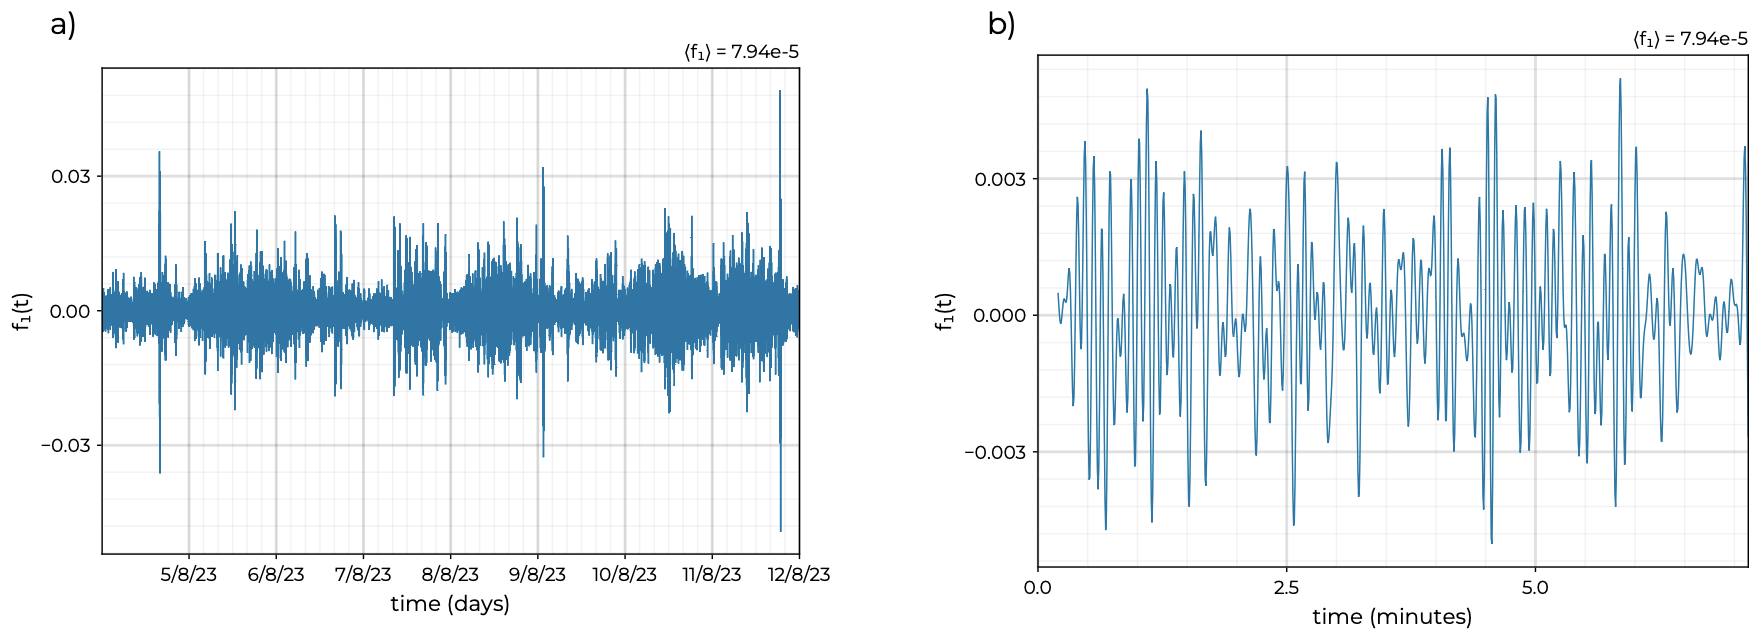
\includegraphics[width=\columnwidth]{havok/2-havok-eval/forcing-time-series.png}
  \caption{(\textbf{a}) Time series of first forcing function activation for the
    duration of the training set. (\textbf{b}) The same time series zoomed in to
    the first 1000 points. The mean value for the forcing function was $7.94\times
    10^{-5}$ reflecting the fact that the learned forcing functions tend to be
    centered about zero with no long-term trend.}
  \label{fig:pm-forcing-time-series}
\end{figure}


To our knowledge, the only other study extending HAVOK for time series
prediction is that of \cite{havok-ml}. In it, the authors use the original
HAVOK formulation from \cite{brunton-havok-orig} under the assumption that
$f(t)$ is linear between time series samples and explored a variety of machine
learning models to predict future $f(t)$ which they then used to construct
forecasts for Lorenz, Mackey-Glass, and Sunspot time series. They found that
tree-based models including Random Forests for the forcing function utilized
with trained HAVOK models yielded better forecasts than methods such
as recurrent neural networks applied directly to the original time series themselves.

For our purposes, we are interested in simple models which could in principle be
deployed on edge computing devices like the single-board computers incorporated
in each sensor node as described in Chapter~\ref{ch:air-network}. This rules out
large models like random forests and deep recurrent neural networks  that would
be challenging to train and deploy at scale for each individual sensor in a
distributed network. Furthermore, our formulation of the HAVOK model involves
\textit{multiple} forcing functions which each must be forecasted. Therefore, we
construct a simple regression model for the entire $\mathbf(f(t+\Delta t))$.
Denoting $\mathbf{z}(t)$ and the current time-delay embedding of PM 2.5 values
and $z(t+\Delta t)$ as the next PM 2.5 value, we fit a model whereby

\begin{equation}
  \mathbf{f}(t+\Delta t) = \mathbf{K}_f\mathbf(f)(t) + \mathbf{K}_{\mathbf{z}}\mathbf{z}(t) + \mathbf{K}_{z}z(t+\Delta t)
\end{equation}

Using the same train-test split as before, the above model achieves an RMSE of
$2.867\times 10^{15}$ on the testing set which is effectively at machine
precision. 


\begin{table}[h]
  \caption{Evaluation of HAVOK forecasting performance as a function of
    prediction horizon from 10 seconds to 4 minutes. \vspace{0.15cm}}
  \label{tab:havok-forecasting-results}
  \centering
  \begin{tabular}{ccccccc} \hline
    \textbf{Duration} & \textbf{RMSE}  & \textbf{RMSE} & \textbf{MAE}   & \textbf{MAE}  & \textbf{MAPE}  & \textbf{MAPE} \\
                      & \textbf{train} & \textbf{test} & \textbf{train} & \textbf{test} & \textbf{train} & \textbf{test} \\\hline
    10 sec.	  & 0.0611 & 0.0589 & 0.0415 & 0.0415 & 0.0054 & 0.0057 \\
    1 min.	  & 0.2555 & 0.2398 & 0.1757 & 0.1720 & 0.0231 & 0.0235 \\
    2 min.	  & 0.7056 & 0.6764 & 0.4874 & 0.4945 & 0.0640 & 0.0674 \\
    3 min.	  & 1.0552 & 1.0366 & 0.7290 & 0.7691 & 0.0957 & 0.1052 \\
    4 min.	  & 1.3759 & 1.3567 & 0.9530 & 1.0185 & 0.1252 & 0.1389 \\
    5 min. 	  & 1.6696 & 1.6530 & 1.1611 & 1.2475 & 0.1525 & 0.1703
  \end{tabular}
\end{table}





\begin{figure}[h]
  \centering
  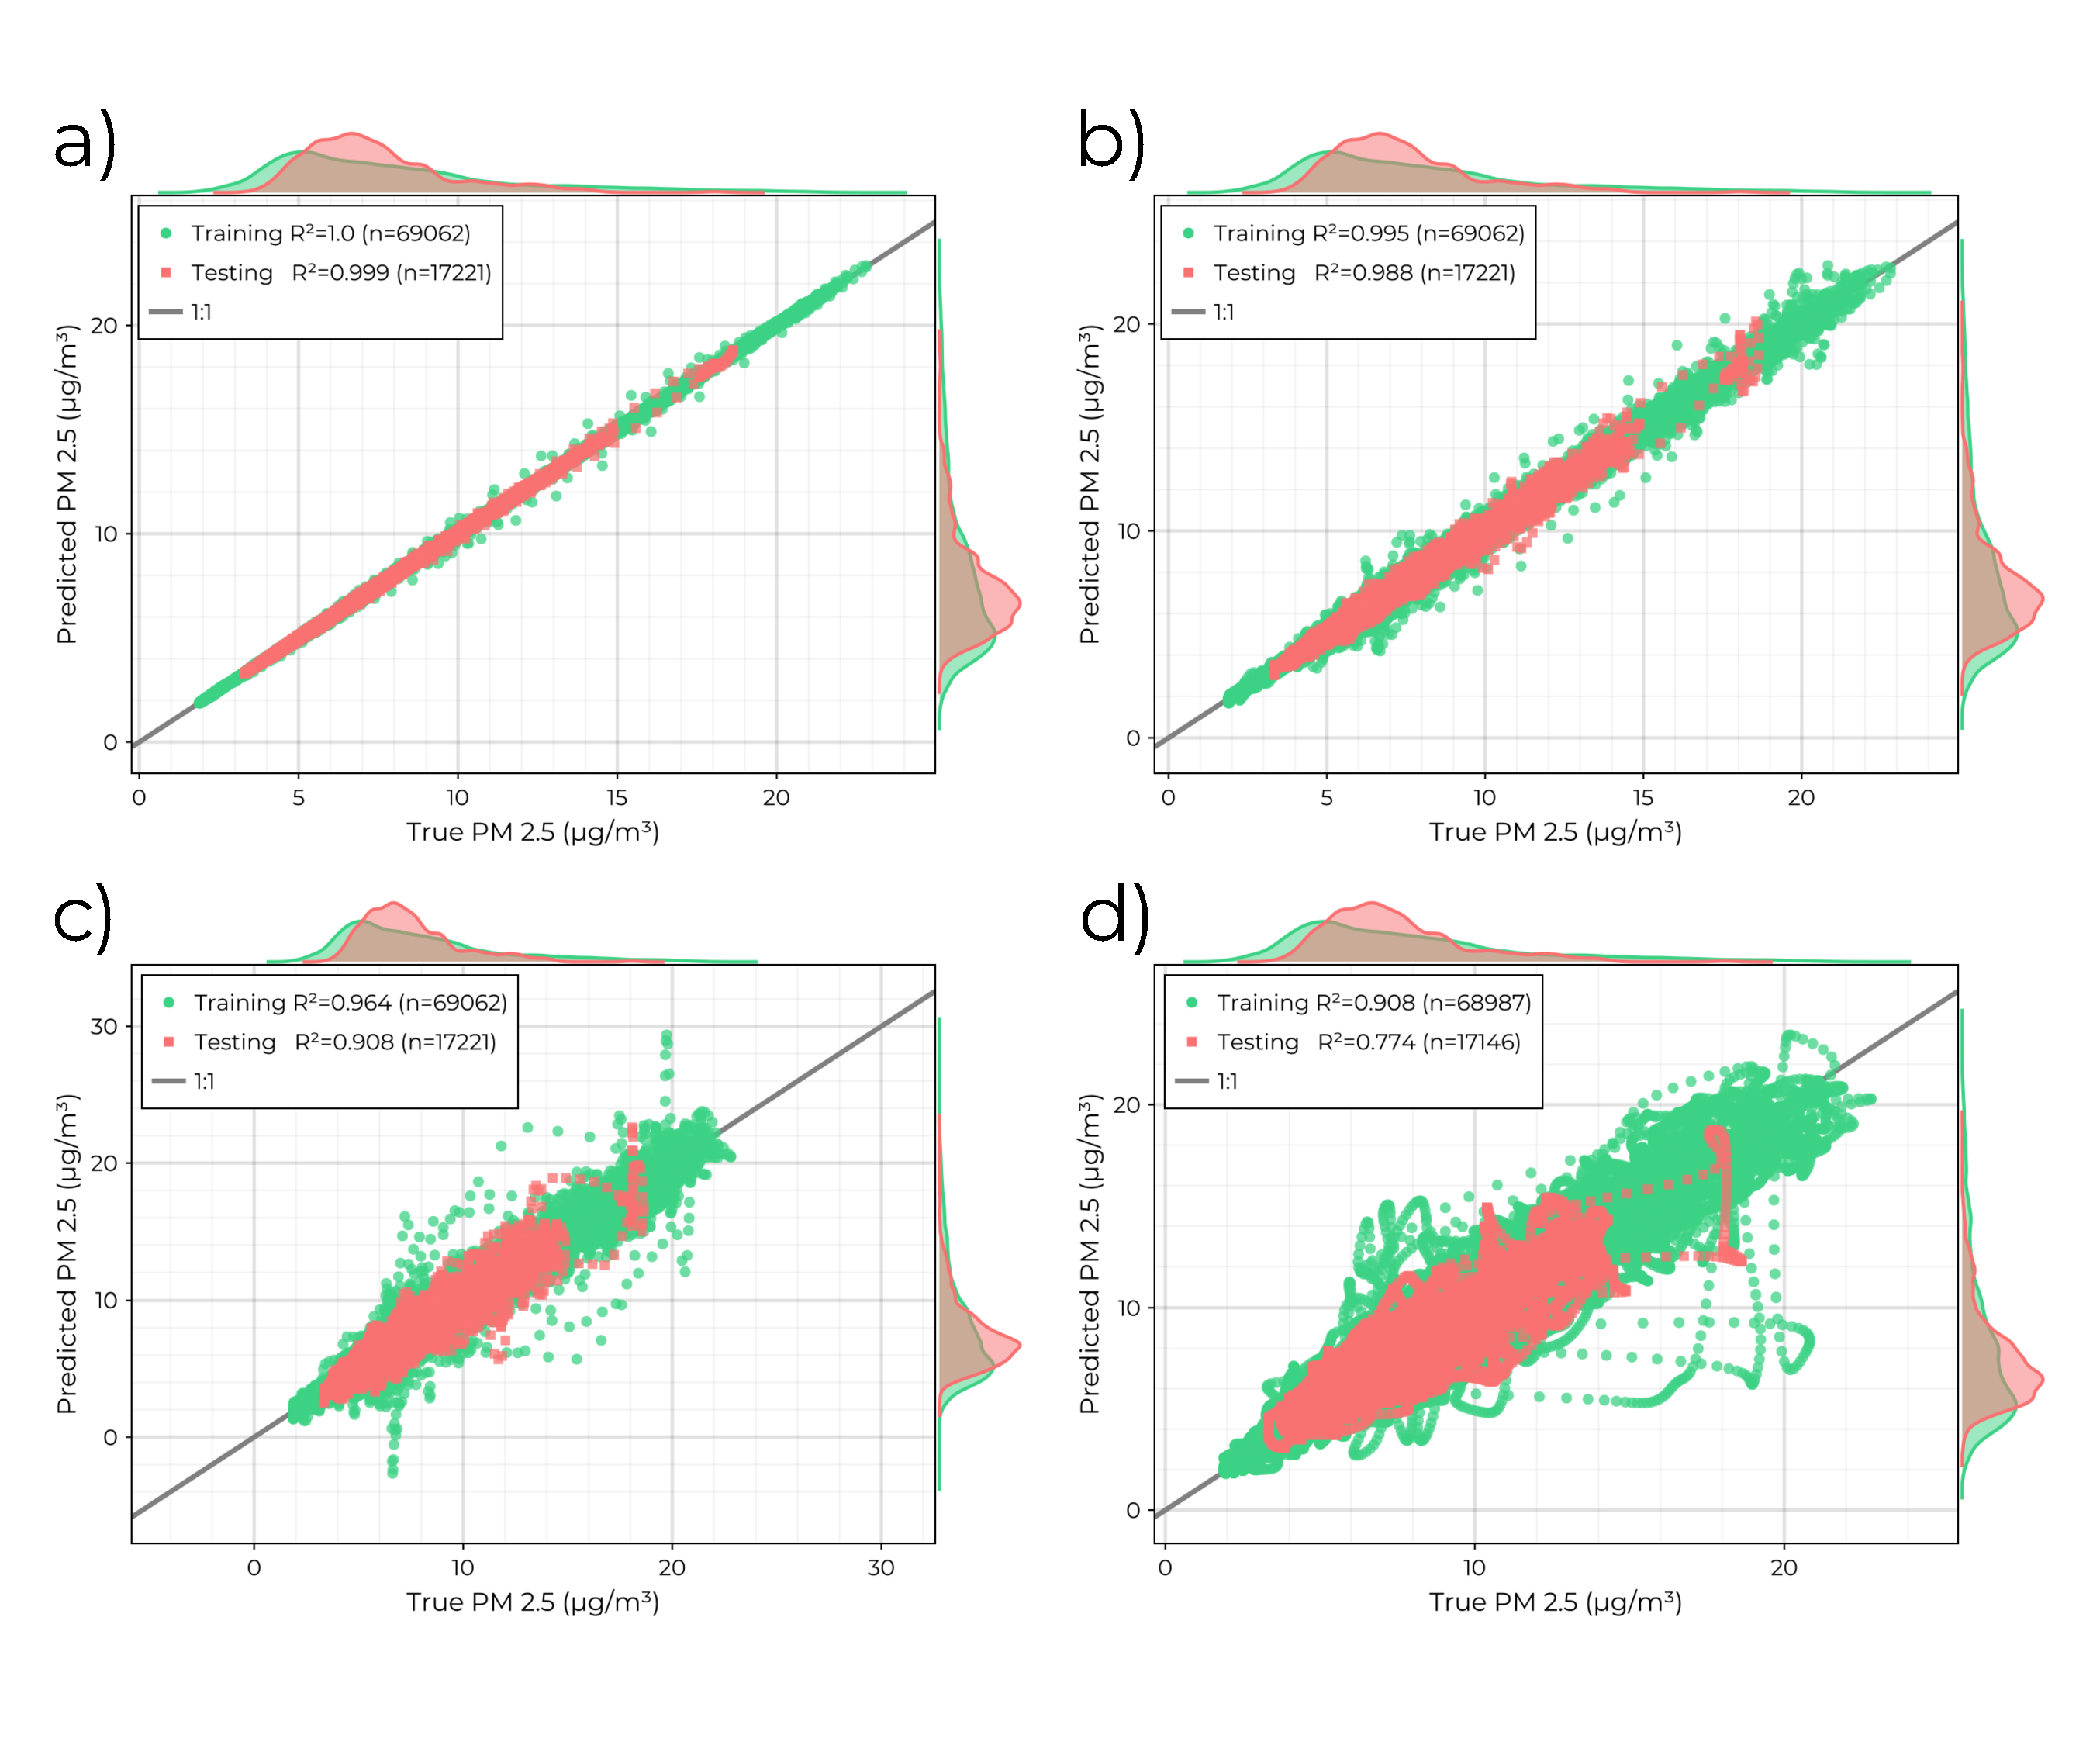
\includegraphics[width=\columnwidth]{havok/3-forcing-fit/forecast-scatter.pdf}
  \caption{Scatter diagrams for multistep forecasts. (\textbf{a}) 10 second
    forecast. (\textbf(b)) 1 minute forecast. (\textbf{c}) 2 minute forecast.
    (\textbf{d}) 5 minute forecast. The integration time step was $\Delta t =
    10$ s so that a 5 minute forecast corresponds to a 30 step future prediction.}
  \label{fig:forecasting-scatter}
\end{figure}

\section{Discussion}

The sHAVOK algorithm is a promising physics-based method which achieves an
attractive compromise between physical motivation and data-driven analysis.
The basic structure of a linear model with intermittent
forcing aligns with known PM trends, namely, the widely observed diurnal cycle
with rare spikes corresponding to brief pollution episodes. The simple structure
of the model also enables efficient fitting for $\mathbf{A}$ and $\mathbf{B}$
using optimized linear algebra routines for the SVD.

- two contributions: use of additional forcing terms and simple procedure for
forecasting the forcing functions, in turn, enabling forecasting of PM

- \cite{havok-ml} also attempted to forecast the forcing function however by
using a simpler integration method assuming piecewise constant forcing, we are
able to generate highly accurate models to predict future forcing values given
the current embedding vector $\mathbf{v}$, the current time delay embedding, and
the \textit{next}, time series values.

- rather than relying on complicated ML models like boosted trees, random
forests, or neural networks to predict the forcing, we are able to achieve
similar results using a simple regression model which.

- combing forecasting of forecasting for forcing terms together with the HAVOK
model enables short-term forecasts for PM 2.5 which are accurate up to 5
minutes. Given that the sampling period used in the study was 10 seconds, a 5
minute prediction corresponds to a 30-step forecast, which far exceeds what
\cite{havok-ml} attempted.

- Thresholding the first forcing function allowed us to accurately identify PM
2.5 spikes suggesting that that is approach may be highly useful for analyzing
historical data. Given the rapidly growing data volume of the sensor network,
the ability to identify aberrant pollution spikes provides useful context when
analyzing bulk PM data.

- Additionally, the forcing function values can be computed whether or not the
HAVOK model is used for forecasting. Since oscillations in the forcing function
tend to precede spikes, HAVOK models trained for each node may be utilized to
provide early warnings for PM spikes for an automated alerting system.
